\documentclass[fleqn,10pt]{wlscirep}
\usepackage{graphicx}
\usepackage{pdfpages}
\usepackage{longtable}
\usepackage{listings}
\usepackage{multicol}
\usepackage{caption}
\usepackage{subcaption}
\PassOptionsToPackage{hyphens}{url}\usepackage{hyperref}
\lstset{
basicstyle=\small\ttfamily,
columns=flexible,
breaklines=true
}
\newcommand{\beginsupplement}{%
        \setcounter{table}{0}
        \renewcommand{\thetable}{S\arabic{table}}%
        \setcounter{figure}{0}
        \renewcommand{\thefigure}{S\arabic{figure}}%
     }

\title{Comparative Annotation Toolkit (CAT) - simultaneous annotation of related genomes}

\author[1]{Ian T. Fiddes}
\author[1,*]{Joel Armstrong}
\author[1,*]{Mark Diekhans}
\author[2,*]{Stefanie Nacthweide}
\author[3]{Zev Kronenberg}
\author[4,5]{Jason Underwood}
\author[3,4]{David Gordon}
\author[6]{Thomas Keane}
\author[3,4]{Evan E. Eichler}
\author[1]{David Haussler}
\author[2]{Mario Stanke}
\author[1,+]{Benedict Paten}
\affil[1]{Genomics Institute, University of California Santa Cruz and Howard Hughes Medical Institute, Santa Cruz, CA 95064, USA}
\affil[2]{Institute of Mathematics and Computer Science, University of Greifswald, Domstraße 11, Germany}
\affil[3]{Department of Genome Sciences, University of Washington School of Medicine, Seattle, WA 98195, USA}
\affil[4]{Howard Hughes Medical Institute, University of Washington, Seattle, WA 98195, USA}
\affil[5]{Pacific Biosciences of California, Inc., Menlo Park, CA 94025, USA}
\affil[6]{European Bioinformatics Institute, Wellcome Genome Campus, Hinxton CB10 1SD, UK}

\affil[+]{Corresponding author. Email: bpaten@soe.ucsc.edu}

\affil[*]{these authors contributed equally to this work}

\keywords{Comparative Annotation, Whole Genome Alignment, Genome Annotation, Comparative Genomics}

\begin{abstract}
The recent introductions of low-cost, long-read and read-cloud sequencing technologies coupled with intense efforts to develop efficient algorithms have made affordable, high-quality \textit{de-novo} sequence assembly a realistic proposition. The result is an explosion of new, ultra contiguous genome assemblies. To compare these genomes we need robust methods for genome annotation. We describe the fully open source Comparative Annotation Toolkit (CAT), which provides a flexible way to simultaneously annotate entire clades and identify orthology relationships. We show that CAT can be used to improve annotations on the rat genome, annotate the great apes, annotate a diverse set of mammals, and annotate personal, diploid human genomes. We demonstrate the resulting discovery of novel genes, isoforms and structural variants, even in genomes as well studied as the rat and great apes, and how these annotations greatly improve cross-species RNA expression experiments. 
\end{abstract}
\begin{document}

\flushbottom
\maketitle
\thispagestyle{empty}

\section*{Introduction}
	We are entering a new era of genome assembly, an era in which high-quality vertebrate and plant sized genome assemblies can be created for many orders of magnitude less money than the original major reference sequencing projects. Short read sequencing prices continue to drop, and new technologies are being developed which move past the shortcomings of short read technologies to produce high quality assemblies \cite{putnam2016chromosome,10xassembly,Jain128835,chaisson2015genetic}. Long read technologies are being leveraged to produce assemblies of quality comparable to those produced through intensive manual curation \cite{gordon2016long} (Kronenberg et al., submitted). These advances have allowed researchers to perform clade genomics, producing assemblies for many members of a single species or related species \cite{Thybert158659,jarvis2014whole}. These advances are required for the ambitious goals of projects such as Genome 10K \cite{haussler2009genome} and Insect 5K, which aim to produce thousands of assemblies for key representative species. In addition, efforts are growing to produce \textit{de-novo} assemblies of individual humans to evaluate the human health implications of structural variation and variation within regions not currently accessible with reference assisted approaches. 
    
These advances in genome assembly require subsequent advances in genome comparison. Central to this comparison is annotation. The challenge of finding functional elements in genome assemblies has been considered for at least the past 20 years \cite{haussler1996generalized}. This problem is traditionally approached by \textit{ab initio} prediction (using statistical models of sequence composition) \cite{stanke2004augustus} and sequence alignment of known mRNAs or proteins\cite{Aken01012016}. The former has limited accuracy while the latter is limited by the existence of useful sequence information. Annotation pipelines such as MAKER \cite{cantarel2008maker}, RefSeq \cite{pruitt2006ncbi} and AUGUSTUS \cite{stanke2006gene} make use of both sequence alignment and \textit{ab-initio} prediction approaches. See \cite{hoff2015current} for a recent review of genome annotation methods. 

A huge amount of effort has gone into the annotation of model organisms, in particular human and mouse. For the past five years, the GENCODE Consortium \cite{harrow2012gencode} has used a wide range of sequencing and phylogenetic information to manually build and curate comprehensive annotation sets, with over 43,281 and 60,297 ORFs in mouse and human, respectively. The GENCODE databases give a glimpse into the diversity of alternative isoforms and non-coding transcripts present in vertebrate genomes. Similarly, efforts in other model organisms such as zebrafish \cite{westerfield1998zebrafish}, \textit{C. elegans} \cite{stein2001wormbase}, \textit{A. thaliana} \cite{swarbreck2008arabidopsis} and many others, have produced high quality annotation sets for their respective assemblies.

As we enter a second era of genome assembly, consideration must also be given to annotating this explosion of assembled, high-quality genomes. Traditional genome assembly projects have been conducted by large consortia with sophisticated in-house annotation pipelines. Individual labs or small groups of labs can now feasibly produce high quality genome assemblies, and tools must be created to give these labs opportunities to produce high quality annotation sets on these assemblies.

Here, we present a method and toolkit to make use of multiple genome alignments produced by progressiveCactus \cite{paten2011cactus} containing one or more previously annotated genomes to simultaneously project well curated annotations onto the lesser studied genomes. In contrast to most earlier alignment methods \cite{blanchette2004aligning,earl2014alignathon,miller200728}, progressiveCactus alignments are not-reference based, include duplications, and are thus suitable for the annotation of many-to-many orthology relationships. We show how the output of this projected annotation set can be cleaned up and filtered through special application of AUGUSTUS \cite{stanke2008using}, and how novel information can be introduced by combining the transitive annotation set with predictions produced by Comparative Augustus \cite{konig2015simultaneous}. These predictions can be further supplemented and validated by incorporating long range RNA-sequencing data such as those generated by the IsoSeq protocol \cite{gordon2015widespread}. We provide a fully featured annotation pipeline, the Comparative Annotation Toolkit (CAT), that can perform this annotation process reproducibly on any combination of a local computer, a compute cluster, or on the cloud with either Amazon Web Services (AWS) or Microsoft Azure. We show that this pipeline can be applied to a wide range of genetic distances, from distant members of the same clade to individualized assemblies of the same species.


\section*{Results}
\subsection*{Comparative Annotation Toolkit}
CAT provides a software toolkit designed to perform end-to-end annotation. The only required inputs are a hierarchical alignment format (HAL) \cite{hickey2013hal} multiple genome alignment as produced by progressiveCactus and a GFF3 format annotation file for the previously annotated genome(s). CAT can take as optional input a set of aligned RNA-seq or IsoSeq BAM format files, as well as protein FASTA files, which are used to construct hints for AUGUSTUS. Based on input parameters, CAT will run AUGUSTUS in up to four distinct parameterizations, two of which rely on transMap projections and two which perform \textit{ab-initio} predictions using extrinsic information to guide prediction. The output of these modes of AUGUSTUS are evaluated alongside the original transMap projections using a combination of classifiers as well as the output from homGeneMapping \cite{stanke2004augustus}. A consensus finding algorithm combines these gene sets (Figure \ref{fig:fig1}). For a more detailed description of CAT and its modules see the cat pipeline detailed description in the supplementary text.

\subsection*{Annotation of great apes}
The previous generation great ape assemblies (panTro4, ponAbe2 and gorGor4) as well as the new SMRT (PacBio) great ape assemblies \cite{gordon2016long} (Kronenberg et al., submitted) were annotated by CAT, using GRCh38 and GENCODE V27 as the reference. CAT identified an average of 141,477 more transcripts and 25,090 more genes in the SMRT assemblies compared to the Ensembl V91 annotation of the older great ape assemblies. Relative to the existing human annotation, the CAT annotations represent an average of 95.0\% of GENCODE gene models and 94.3\% of GENCODE isoforms in the SMRT great ape assemblies. Comparing the CAT annotations of SMRT assemblies to the legacy assemblies, we see an average increase of 610 genes (1.9\%) and 3,743 isoforms (1.0\%) (Supplemental Figure \ref{supp_fig:primate_completeness}); most of the observed increase in genes and isoforms relative to the Ensembl annotations are therefore a result of the CAT annotation process rather than the updated assemblies.

% Move this to supplement: (a pre-release of Ensembl V91 was provided to us for chimpanzee and gorilla). 
Conversely to the overall increases in genes and isoforms, CAT identifies on average 3,553 fewer protein coding genes than Ensembl. However, this brings the total number of coding genes more closely in line with the GENCODE annotation of human, as Ensembl has an average of 2,081 more protein coding genes in great apes than GENCODE has for human (Supplemental Figure \ref{supp_fig:primate_completeness}). 

To evaluate these annotations in a non species-biased fashion, consensus isoform sequences created from IsoSeq reads for each species were compared to their respective species annotations. As a baseline comparison, equivalent human data was compared to the high-quality human GENCODE V27 annotation. The CAT annotation of both the SMRT and legacy great ape assemblies (which used the raw IsoSeq reads during the annotation process), and the Ensembl annotation of the legacy assemblies were compared. We calculated the rate of isoform concordance, that is the fraction of consensus IsoSeq sequences that match either exactly or fuzzily an annotated isoform (Figure \ref{fig:fig2}A; methods). Fuzzy matching allows for the intron boundaries to shift slightly in a isoform. For the SMRT chimpanzee (74.0\%/82.1\% exact/fuzzy matching) and orangutan (71.4\%/80.4\%) genome assemblies the isoform conordance rates were comparable to the rate for human (74.6\%/82.1\%) with the exception of the gorilla GSMRT3.2 assembly (67.6\%/76.9\%), likely due to the higher indel error rate in that assembly (Supplemental Figure \ref{supp_fig:primate_indels}). In contrast, the isoform concordance rate for the legacy assemblies was lower (on average 60.0\%/69.6\%), mostly reflecting exons in gaps and mis-joins, and was lower still for the existing Ensembl annotations (on average 47.9\%/57.6\%).

To further assess the utility of CAT annotations for the analysis of RNA expression, species-specific iPSC Illumina RNA-seq data were quantified against the great ape assemblies, with both CAT and Ensembl annotations for the older assemblies (Figure \ref{fig:fig2}B). 
% Check numbers in this sentence 
Comparing the annotations of the older assemblies, CAT identified an average of 9,518 more genes and 54,107 more transcripts with measurable expression compared to Ensembl.
We might expect the per-gene abundance estimates of the majority of genes in matched cell types to agree between species, particularly for closely related species. It is reasonable to therefore prefer \textit{a priori} an annotation of the great apes that produces expression estimates that agree with expression estimates from the matched human data using the high-quality GENCODE annotation. Doing this comparison separately using the CAT and Ensembl annotations, we find better correlations using the CAT annotations (avg. Pearson r=0.63; \ref{fig:fig2}D, Supplemental Figure \ref{supp_fig:primate_expression}) than the Ensembl annotations of the older assemblies (avg. Pearson r=0.43) for gorilla and orangutan. However, we find by far the highest correlation when CAT annotates the SMRT primate assemblies (avg. Pearson r=0.90). This reflects the increased representation in the updated assemblies of transcript sequence, especially 3' UTR regions that are important for quantifying polyA primed RNA-seq (Kronenberg et al., submitted). Notably, we find that the correlations between the CAT annotations of the SMRT assemblies and the matched human data are higher than when mapping the species specific data back to the human GENCODE annotations and comparing to the human data, despite the maturity of the human annotation, suggesting that mappability issues play a role.

Predictions performed by AugustusCGP and AugustusPB were incorporated into the gene sets based on the presence of splice junctions supported by RNA-seq or IsoSeq and not present in the transMap/AugustusTMR derived annotations (Figure \ref{fig:fig2}C). An average of 1,677 novel isoforms and 64 novel loci were found across the assemblies with at least one IsoSeq read supporting the prediction.

CAT provides new metrics for diagnosing assembly quality. In the process of annotating the great ape genomes, we noticed that assemblies that had undergone Quiver and Pilon \cite{walker2014pilon} correction still exhibited a systematic bias towards coding deletions. These were identified to be related to heterozygosity in the input dataset, and a variant calling based correction method (Kronenberg et al., submitted) was developed to resolve these issues, dramatically lowering the coding indel rate and reducing systematic bias (Supplemental Figure \ref{supp_fig:primate_indels}).

CAT can also diagnose assembly contiguity by reporting the number of genes whose transcripts end up split across multiple contigs, or on disjoint intervals in the same contig. Comparison of split gene metrics between the old and new primate assemblies shows 504 fewer split genes in chimpanzee, 560 fewer in gorilla and 1,858 fewer in orangutan (Supplemental Figure \ref{supp_fig:primate_split_genes}).


\subsection*{Annotation of personal human diploid assemblies}
High-quality de novo assembly of a human genome is increasingly feasible; both Pacific Biosciences \cite{chin2016phased,huddleston2016discovery,korlach2017novo} and 10x Genomics \cite{Weisenfeld070425} provide tools to construct phased, diploid assemblies. Annotating diploid assemblies provides a window into haplotype-specific structural variation that may affect gene expression. To evaluate the ability of CAT to provide this analysis a progressiveCactus alignment was generated between hg38 and the two haploid cell line assemblies, CHM1 (GCA\_001297185.1) and CHM13 (GCA\_000983455.2), and CAT used to annotate the resulting pseudo-diploid CHM1/CHM13 genome in the alignment. 99.3\% of genes present in GENCODE V27 were identified in CHM1, and 99.2\% in CHM13 (Figure \ref{fig:fig3}A). 
    
	After filtering, 733 genes in CHM1 and 585 genes in CHM13 were identified with frame-shifting indels. Compared to ExAC, which found between 75 and 125 putative truncating events per individual \cite{karczewski2016exac}, this result suggests indel errors in the assemblies are producing false positives. Both assemblies exhibit a systematic over-representation of deletions despite coming from haploid cell lines (Figure \ref{fig:fig3}B, left). Split gene analysis found the CHM1 assembly to be slightly more gene contiguous (Figure \ref{fig:fig3}B, right).

Manual analysis of the 27 genes missing in CHM13 relative to CHM1 and the 6 genes missing in CHM13 relative to CHM1 led to the discovery of the example region in figure \ref{fig:fig3}C. This deletion removes most of the exons of TRIB3, a pseudokinase associated with type 2 diabetes \cite{shi2009association} (Supplemental Figure \ref{supp_fig:trib3}).


\subsection*{Annotation of a diverse set of mammals}
	13 mammalian genomes were comparatively annotated using mouse (mm10) as the reference, and GENCODE VM15 as the source transcript set. Species-specific RNA-seq was used for every genome (Supplemental Table \ref{supp_table:rnaseq_sra_table}). To assess the quality of these annotation sets, 4,104 benchmarking universal single copy orthologs (BUSCO) were used \cite{simao2015busco}. On average, only 108 BUSCO genes (2.63\%) were missing in each genome  (Figure \ref{fig:fig4}A). Only three BUSCO genes (EOG090A0GHJ, EOG090A05ND, and EOG090A04MN) were missing in all of the target genomes, while 832 were missing in at least one genome. Gene ontology enrichment analysis of the 271 genes missing in two or more genomes had only one hit, cellular component organization (p=1.02e-3, 1.57 fold enrichment). 555 BUSCO genes were missing in only one genome (Supplemental Figure \ref{supp_fig:busco_missing}). These data, combined with the lower value seen in human suggest that there is not a systematic bias in the genes missing but rather a result of a combination of assembly quality and alignment errors.

To estimate the usefulness of these annotation sets, the input RNA-seq datasets were used to quantify expression of the annotation sets (Figure \ref{fig:fig4}B). The main factor in measurable expression is the variety of the input RNA-seq datasets, as exemplified by the ability to measure expression of 88.9\% of genes annotated in the sheep genome. On average, 6,739 coding genes, or 35.6\% of the coding genes in each genome had paralogous alignments that were resolved. The rate of paralogy did not vary noticeably with phylogenetic distance (Figure \ref{fig:fig4}C)).


\subsection*{Reannotating the rat genome}
	CAT was run on a Cactus alignment between mouse (mm10) and rat (rn6) using rabbit (oryCun2), Egyptian jerboa (jacJac1) and human (hg38) as outgroups. To provide hints to AUGUSTUS, RNA-seq data were obtained from SRA \cite{fushan2015gene,cortez2014origins,liu2016identification} (Supplemental Table \ref{supp_table:rnaseq_sra_table}). CAT comparatively annotated 78.1\% of genes and 91.9\% of protein coding genes present in GENCODE VM11 on rn6 (Supplemental Figure \ref{supp_fig:rat_completeness}), representing an increase of 14,675 genes and 74,308 transcripts over Ensembl V90 and 5,104 genes and 32,157 transcripts over RefSeq. 13,651 loci were identified with no overlap to any other annotation set (Supplemental Figure \ref{supp_fig:rat_locus_venn}).
    
The input RNA-seq dataset was used for isoform quantification against the CAT, MAKER, Ensembl and RefSeq transcriptomes (Figure \ref{fig:fig5}B). CAT identified 1,881 protein coding genes and 1,011 lncRNAs with measurable expression not present in either Ensembl or RefSeq. CAT also identified 27,712 expressed coding splice junctions not in the union of RefSeq and Ensembl, for a total of 21,267 novel expressed isoforms.

For comparison the MAKER pipeline \cite{cantarel2008maker} was run in parallel. MAKER was provided both a Trinity \cite{haas2013novo} \textit{de-novo} assembly of the input RNA-seq data provided to CAT (it does not process raw RNA-seq) as well as the mouse protein sequences from GENCODE VM11, together providing a comparable input set to what CAT had. 

19,817 of CAT loci and 17,163 of MAKER loci overlapped the union of Ensembl and RefSeq (Supplemental Figure \ref{supp_fig:rat_locus_venn}). The exact matches of CDS exons and CDS introns were compared (Supplemental Figure \ref{supp_fig:rat_exon_intron}). For both CDS exons and CDS introns, both Ensembl and RefSeq displayed the highest Jaccard (intersection / union) similarity, followed by CAT and the two reference annotation sets (Figure \ref{fig:fig5}A).

AugustusTMR, which uses TransMap and RNA-seq, provides CAT with a way to improve transcript projections, which we quantify via RNA-seq mapping (Supplemental Figure \ref{supp_fig:augustus_rna_rat}).


\subsection*{CAT annotations over large phylogenetic distance}
To show that CAT can work across large phylogenetic distances, the annotation of human GRCh37 produced in the representative mammalian genome annotation was compared to the current human GENCODE annotation set (GENCODE V27lift37). The Jaccard similarity of the CAT annotation to GENCODE annotation set was similar to the similarities seen in the rat comparison (Figure \ref{fig:fig5}C). The two annotation sets were compared using Kallisto with a human iPSC RNA-seq dataset that was not used in the annotation process. Kallisto was able to detect expression of 13,765 protein coding genes and 38,464 protein coding transcripts from the CAT annotation (Figure \ref{fig:fig5}D). Of the 19,233 ICE isoforms detected when running ToFu \cite{gordon2015widespread} against hg19, 12,911 (67.15\%) fuzzy matched a CAT isoform compared to 15,920 (82.8\%) of GENCODE V27lift37 (Figure \ref{fig:fig5}E). The detection of alternative isoforms across large phylogenetic distance can improve comparative genomic analysis in upcoming large scale comparative genomics projects like the Vertebrate Genomes Project \cite{haussler2009genome} (\url{http://www.sanger.ac.uk/science/data/vertebrate-genomes-project}).

\section*{Discussion}
Gene annotation is a longstanding and critical task in genome informatics that must now be scaled to handle the rapidly increasing number of available genomes. CAT performs better than existing annotation pipelines by leveraging existing annotation sets, both long and short read RNA-seq data, protein information, and state of the art single- and multi-genome predictions developed by our group. CAT produces consistent annotation sets of many genomes within a clade with minimal reference bias. This result is clearly shown in the analysis of the rat genome, where more genes and many more transcripts are detectable in RNA expression analysis than when using other annotation methods, including the standard, popular reference annotations from Ensembl and RefSeq.

Provided with sufficient extrinsic data, CAT provides a way to generate an unbiased annotation set across a clade. The extensive RNA-seq and IsoSeq data provided in the primate annotation led to the discovery of splice junctions and exons not present in the human genome. CAT can detect structural variants with gene expression effects in personal human genomes through analysis of genes either missing or incompletely mapped.

CAT provides a framework for leveraging existing high-quality annotation efforts such the GENCODE effort. For example, the analysis of the rat genome shows that many of the alternative isoforms and projected transcription start sites identified by GENCODE in mouse are supported by expression analysis in rat (Supplemental Figure \ref{supp_fig:unsupported_junctions}). Supporting the quality of the created annotation, isoform concordance between CAT and Genbank mRNAs is much greater than MAKER, and comparable to Ensembl. However, the nevertheless relatively low rate of concordance speaks to the difficulty in fully annotating isoforms, especially UTR exons. 

GENCODE has spent considerable effort over the past few years re-classifying protein-coding loci as pseudogenes, lincRNA and other non-coding biotypes. These false positives are inherent in the nature of gene finding tools, where the likelihood of finding a valid but apparently non-conserved ORF in a given transcribed locus is not small \cite{lin2011phylocsf}. CAT provides a way to bypass this inherent challenge in gene finding by leveraging the existing information in an annotation set like GENCODE, and as a result identified an average of 18,364 coding genes in the legacy great apes compared to an average of 21,918 in Ensembl. If a transcript’s biotype is incorrect in the input set, CAT currently has no way of re-evaluating this, but in the future we hope to add processed, unprocessed and unitary pseudogene prediction to CAT.

CAT is not without limitations. In addition to the problem of opaque biotypes, there are trade-offs to be made over genetic distance in regards to conservation of alternative isoforms. Tuning the flags related to RNA-seq support can filter out non-conserved isoforms, but also makes the assumption that the given RNA-seq data are comprehensive. We also would like to integrate coding potential prediction\cite{lin2011phylocsf} to both our novel predictions as well as projection transcripts. 

CAT works best when provided RNA-seq data, but for many species this may not be possible. From our experience, a reasonable amount (on the order of 50 million reads) of RNA-seq from tissues like brain and liver is fairly informative. Using polyA selected libraries is recommended, as it greatly reduces false positive predictions in AugustusCGP. IsoSeq data allowed for the discovery of thousands of novel isoforms in the great apes, but may be too expensive for many projects. In clade genomics projects, we would suggest generating RNA-seq for a few of the species and then rely on the coordinate mapping that AugustusCGP and homGeneMapping provide to evaluate support in other members of the clade.

File formats can also be a practical limitation. CAT produces annotations in both the genePred and GFF3 format. We have included a script to convert these annotations into a format suitable for submission at NCBI. However, compromises have to be made in how to best represent frame-shifts found relative to the source transcript set that are ambiguous with regards to assembly error or true biology.

An earlier version of CAT was used to annotate the PacBio-based assembly of the gorilla genome \cite{gordon2016long} as well as produce the current Ensembl annotations for 16 laboratory mouse strains as part of the Mouse Genomes Project (\url{http://www.sanger.ac.uk/science/data/mouse-genomes-project}). In addtion, CAT has been proposed for the Vertebrate Genomes Project (VGP), which aims as a pilot project to assemble and annotate one member of every order of vertebrate species. CAT also will be used on the 200 Mammals Project, which aims to add approximately 140 new mammalian genome assemblies to the existing set. These projects will provide a new understanding of gene evolution.

CAT’s current implementation does not attempt to put weights on the features used for constructing a consensus gene set. Instead, it simply scores transcripts based on the sum of all features evaluated. In the future deep learning methods could be added to CAT to construct feature weights and improve consensus finding, and so better mimic the labor intensive efforts of manual annotators who currently weigh such evidence.

\section*{Materials and Methods}
CAT produces as output a series of diagnostic plots, an annotation set for each target genome, and a UCSC comparative assembly hub \cite{nguyen2014comparative}. Both the pipeline and associated documentation can be found at \url{https://github.com/ComparativeGenomicsToolkit/Comparative-Annotation-Toolkit}. CAT is constructed using the Luigi (\url{https://github.com/spotify/luigi}) workflow manager, with Toil \cite{vivian2017toil} used for computationally intensive steps that work best when submitted to a compute cluster. 

\subsection*{RNA-seq}
CAT annotation is improved when species-specific RNA-seq data are provided. These data are used as hints for AugustusTMR and AugustusCGP. In AugustusTMR, RNA-seq helps fill in missing information in the alignment, as well as resolve evolutionary changes. In AugustusCGP, RNA-seq additionally helps prevent false positives inherent in \textit{ab-initio} gene finding. For these reasons, RNA-seq was obtained from SRA for all species annotated in this paper. All RNA-seq were aligned to their respective genomes with STAR \cite{dobin2013star} and the resulting BAM files passed to CAT to construct the extrinsic hints database. See Table \ref{table:tables1} for accessions and tissue types of RNA-seq data used for annotation. In addition, for the PacBio great ape annotation, RNA-seq data were generated using iPS cell lines for human, chimpanzee, gorilla and orangutan derived from cells for the same individuals as the assemblies (Kronenberg et al., submitted). For all expression analyses, Kallisto \cite{bray2015near} was used.

\subsection*{Annotation set similarity analysis}
Jaccard similarity analysis was performed with bedtools \cite{quinlan2010bedtools}. The rat locus overlap analysis was performed with the Kent tool clusterGenes, which requires exonic overlap on the same strand.

\subsection*{IsoSeq}
IsoSeq full-length non-chimeric reads (FLNC) were also generated from the great ape iPSC lines and aligned with GMAP \cite{wu2005gmap}.To perform isoform level validation in the primates, the IsoSeq data used as input to CAT were also clustered with isoform-level clustering (ICE) and then collapsed into isoforms using ToFu \cite{gordon2015widespread}. Ensembl provided a pre-release of their new V91 annotations for panTro4 and gorGor4, but did not yet run their updated pipeline on ponAbe2.

\subsection*{ICE validation}
The output transcripts from ICE were compared to various annotation sets in both an exact and fuzzy matching scheme. In the exact scheme, the genomic order and positions of all of the introns (an intron chain) of a transcript are compared to any ICE isoforms which overlap it. In the fuzzy matching scheme, each annotated intron chain is allowed to move up to 8 bases in either direction and still be called a match.

\subsection*{BUSCO}
The mammalian BUSCO analysis was performed using the mammalia\_odb9 set of 4,104 genes. BUSCO was ran against the complete protein coding sequence repertoire produced by CAT in that species in the `protein' mode.

\subsection*{progressiveCactus}
	All cactus alignments except the 14-way mammal alignment were generated using progressiveCactus (\url{https://github.com/glennhickey/progressiveCactus}) commit 91d6344. For the mouse-rat alignment the guide tree was 

\begin{lstlisting}
(((Lesser_Egyptian_jerboa:0.1,(Mouse:0.084509,Rat:0.091589)mouse_rat:0.107923)rodent:0.148738,Rabbit:0.21569)glires:0.015313,Human:0.143908);
\end{lstlisting}
    
For the primate alignments, the guide tree was 
    
\begin{lstlisting}
(((((((Susie_Gorilla:0.008964,(Human:0.00655,Clint_Chimp:0.00684)human_chimp:0.00122)gorilla_chimp_human:0.009693,Susie_Orangutan:0.01894)great_ape:0.003471,Gibbon:0.02227)great_ape_gibbon:0.01204,Rhesus:0.004991)old_world_monkey:0.02183,Squirrel_monkey:0.01035)monkey:0.05209,Bushbaby:0.1194)primate_anc:0.013494,Mouse:0.084509);
\end{lstlisting}
    
An identical tree (with different assembly names) was used for the alignment of current reference great apes. For the pseudo-diploid human alignment, the guide tree was 
    
\begin{lstlisting}
((hg38:0.001,chm1:0.001,chm13:0.001)human:0.01,chimp:0.01);
\end{lstlisting}
    
representing a star phylogeny of the three human assemblies. For the 14-way mammal alignment, the progressiveCactus commit used was e3c6055 and the guide tree was 
    
\begin{lstlisting}
((((oryCun2:0.21,((Pahari_EiJ:0.03,mm10:0.025107)1:0.02,rn6:0.013)1:0.252)1:0.01,((((hg19:0.00642915,panTro4:0.00638042)1:0.00217637,gorGor3:0.00882142)1:0.00935116,ponAbe2:0.0185056)1:0.00440069,rheMac3:0.007)1:0.1)1:0.02,((oviAri3:0.019,bosTau8:0.0506)1:0.17,(canFam3:0.11,felCat8:0.08)1:0.06)1:0.02)1:0.02,loxAfr3:0.15);
\end{lstlisting}
    
    
Slightly out-of-date versions of some assemblies (hg19 and rheMac3) were used because a collaborator had data on those assemblies that they wished to use the alignment to analyze. The rodent and primate subtrees were first aligned separately (the rodent subtree originally included additional mouse strains). The two subtrees were then “stitched” together into a single alignment by aligning together their roots along with several Laurasiatheria genomes. This was done to save alignment time by reusing existing alignments.

\subsection*{CAT}
CAT was ran on the UCSC Genome Browser compute cluster for all annotation efforts in this publication. CAT commit f89a814 was used. For a detailed description of how CAT works, see both the supplementary text as well as the README.md on github (\url{https://github.com/ComparativeGenomicsToolkit/Comparative-Annotation-Toolkit}). 

\subsection*{Pipeline runtime}
CAT is relatively efficient, taking on the order of thousands of core hours to run. The largest considerations for runtime are running the various parameterizations of AUGUSTUS. AugustusCGP may run significantly faster on alignments with many genomes by reducing the chunk size from the default, but at the cost of lower quality predictions. AugustusTMR runtime scales linearly with the number of protein coding genes in the input annotation set, but scales non-linearly with the number of extrinsic hints provided, particularly if the hints are contradictory. 
Running CAT on the PacBio primate genomes took a total of 7,030 core hours, with 3,437 of those dedicated to running AugustusTMR, 1,191 dedicated to running AugustusPB, and 2,190 dedicated to running AugustusCGP. Running CAT on the 14-way mammalian alignment took a total of 24,122 core hours, with 14,045 of those dedicated to running AugustusTMR, and 8,225 dedicated to running AugustusCGP.

\section*{Acknowledgements}
We would like to thank Brian Raney, Hiram Clawson and the rest of the UCSC Browser team for help creating browser tracks, and Dent Earl, whose work led to this project. We also would like to thank Fergal Martin and Paul Flicek for revising the paper and providing a pre-release of the Ensembl V91 annotations on chimpanzee and gorilla.

\bibliography{references}
\clearpage

\begin{figure}
\centering
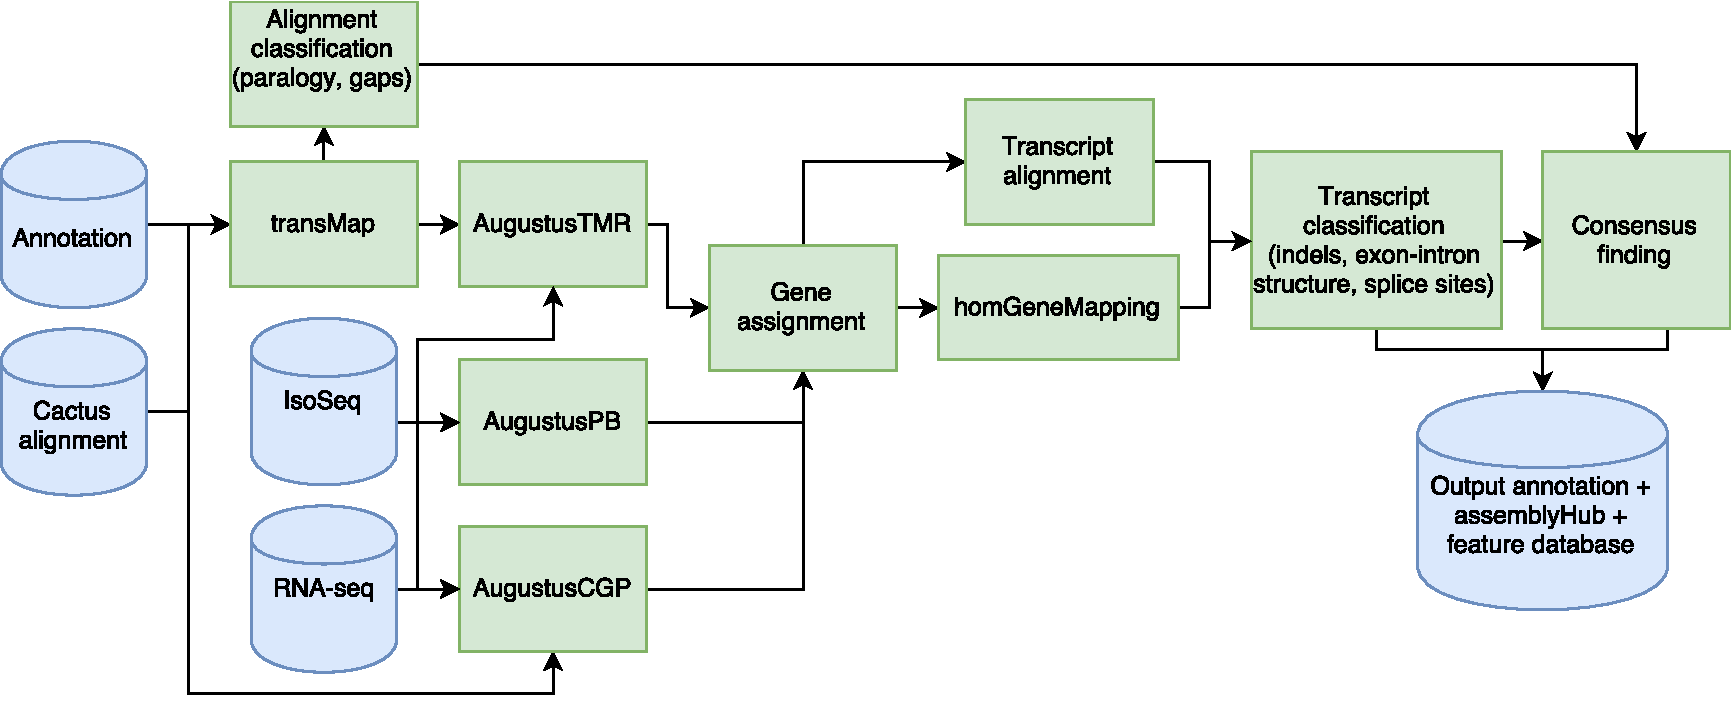
\includegraphics[width=\textwidth,height=\textheight,keepaspectratio]{CAT.pdf}
\caption{CAT pipeline schematic}
The CAT pipeline takes as input a HAL alignment file, an existing annotation set and aligned RNA sequencing reads. CAT uses the Cactus alignment to project annotations to other genomes using transMap \cite{stanke2008using}. These transcript projections are then filtered and classified. Optionally, AUGUSTUS can be run into up to three parameterizations. 1) AugustusTMR, treats each transcript projection separately and fixes errors in projection. 2) AugustusPB, uses long read RNA sequencing to look for novel isoforms. 3) AugustusCGP \cite{konig2015simultaneous} uses the Cactus alignment to simultaneously predict protein coding genes in all aligned genomes. CGP and PB predictions are assigned to transMap projections where possible. All transcripts are classified for extrinsic support and structure and a ‘chooser’ algorithm picks the best representative for each input transcript, incorporating CGP and PB transcripts when they provide novel supported information. The final consensus gene set as well as associated feature tracks are used to create a assembly hub ready to be loaded by the UCSC browser.
\label{fig:fig1}
\end{figure}

\begin{figure}
\centering
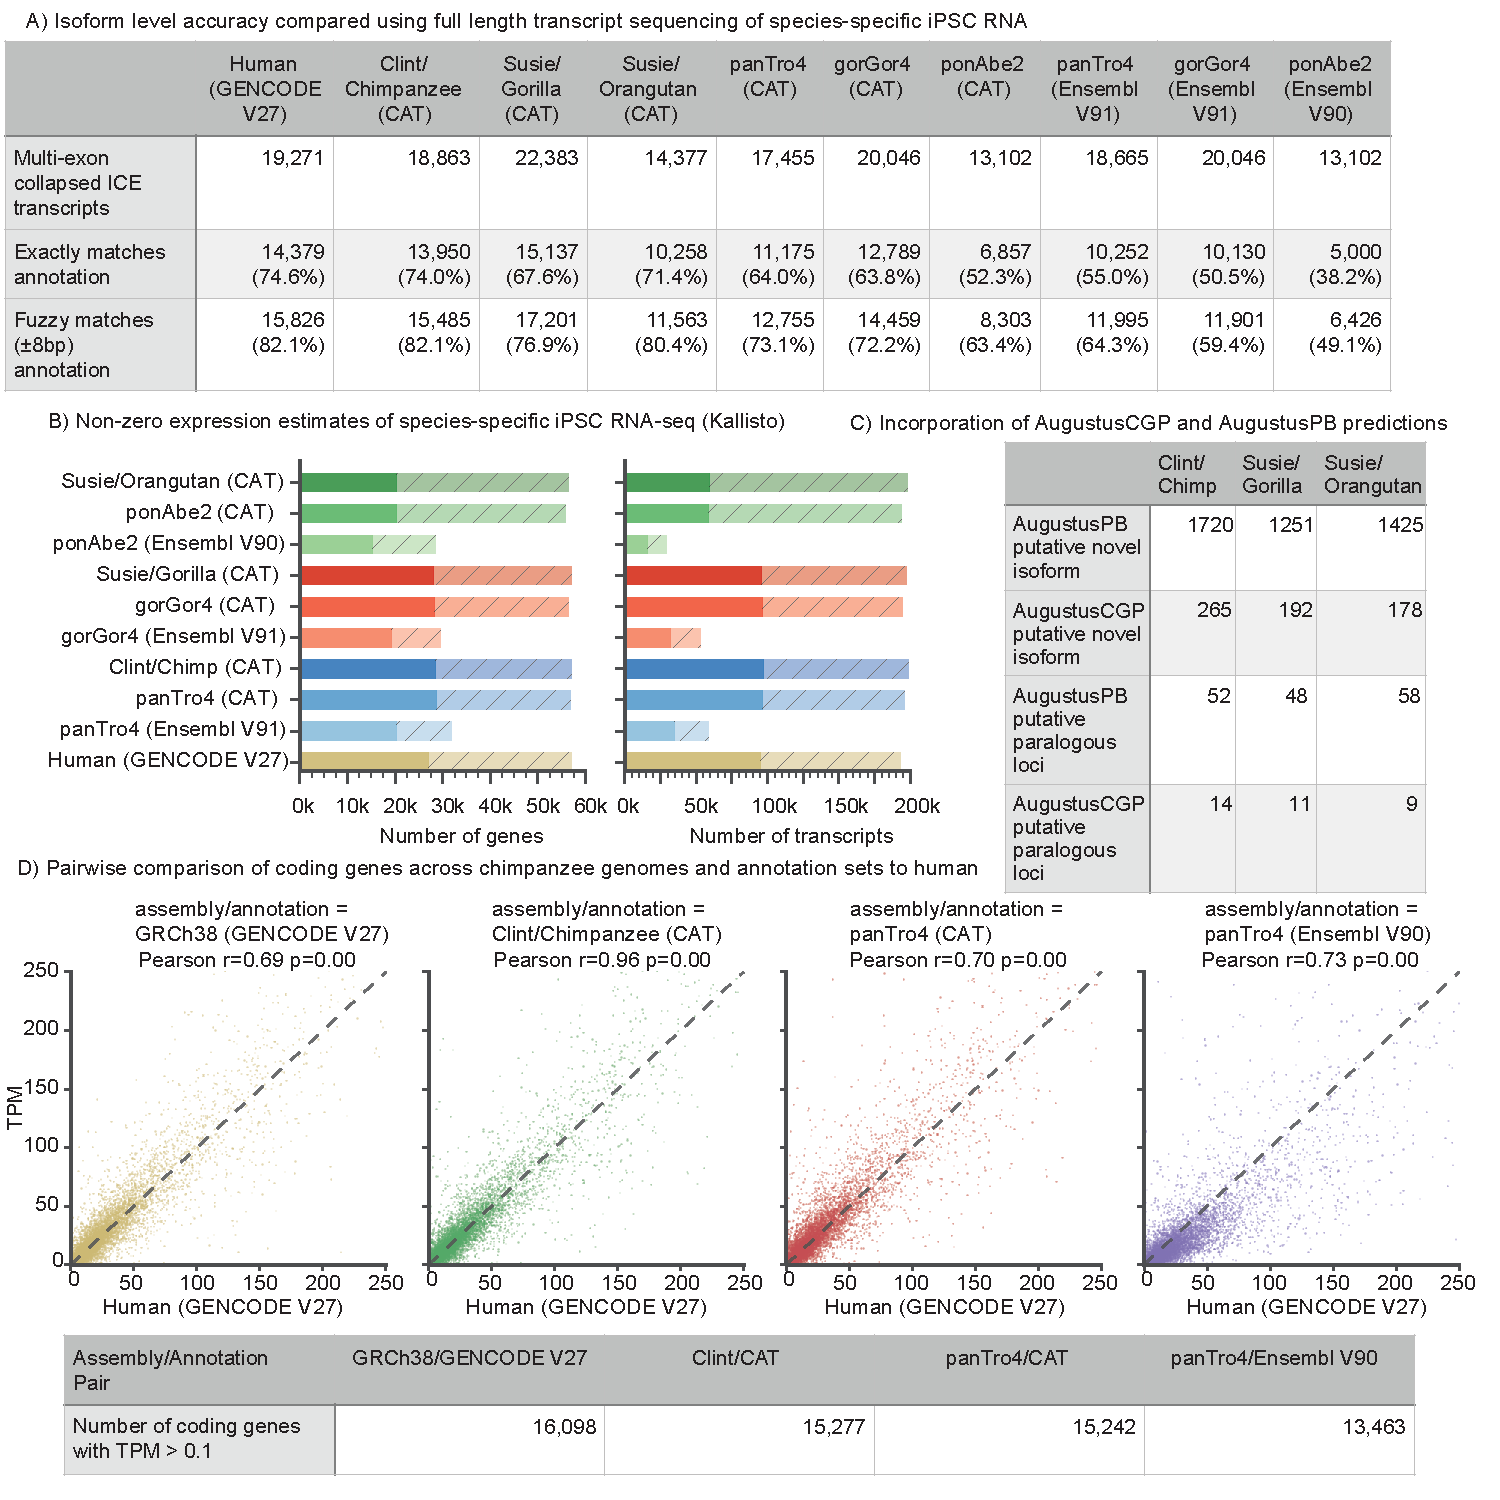
\includegraphics[width=0.8\textwidth,height=0.8\textheight,keepaspectratio]{figure2-primate_v9.pdf}
\caption{Primate annotation}
A) Validating CAT annotations using IsoSeq data. As a baseline comparison, IsoSeq data from human iPSC cells were compared to the GENCODE V27 annotation. This provides an upper boundary for how well CAT can perform. IsoSeq data from chimpanzee,  gorilla and orangutan iPSC lines were compared to each respectively, matching CAT genome annotation.  The IsoSeq data were clustered with ICE and collapsed using ToFu\cite{gordon2015widespread}. CAT annotation of PacBio great apes showed similar isoform concordance to human, and improvement over the legacy assemblies. B) Kallisto\cite{bray2015near} was used to quantify liver RNA-seq from each species on both the gene and transcript level on the existing and new great ape assemblies. Solid bars are transcripts or genes with TPM \textgreater 0.1, while shaded hatched bars are the remainder of the annotation sets. CAT annotation of great apes show nearly the same number of expressed genes and isoforms as the GENCODE reference on human with the exception of orangutan. C) The number of novel splices and exons discovered by analysis of AugustusPB predictions for each species. Novel splices have overlap with a comparatively annotated exon, while novel exons have no overlap. Putative paralogous loci are AugustusCGP or AugustusPB predictions with exonic overlap to transMap projections filtered out during paralog resolution. These were filtered by requiring IsoSeq support. D) Kallisto protein coding gene-level expression for chimpanzee iPSC RNA-seq is compared to human across all of the chimpanzee annotation and assembly combinations as well as when mapped directly to human. In all cases the x-axis is the TPM of human iPSC data mapped to human. The highest correlation (Pearson r=0.96) is seen when comparing Clint annotated with CAT to GRCh38 annotated with GENCODE V27.
\label{fig:fig2}
\end{figure}

\begin{figure}
\centering
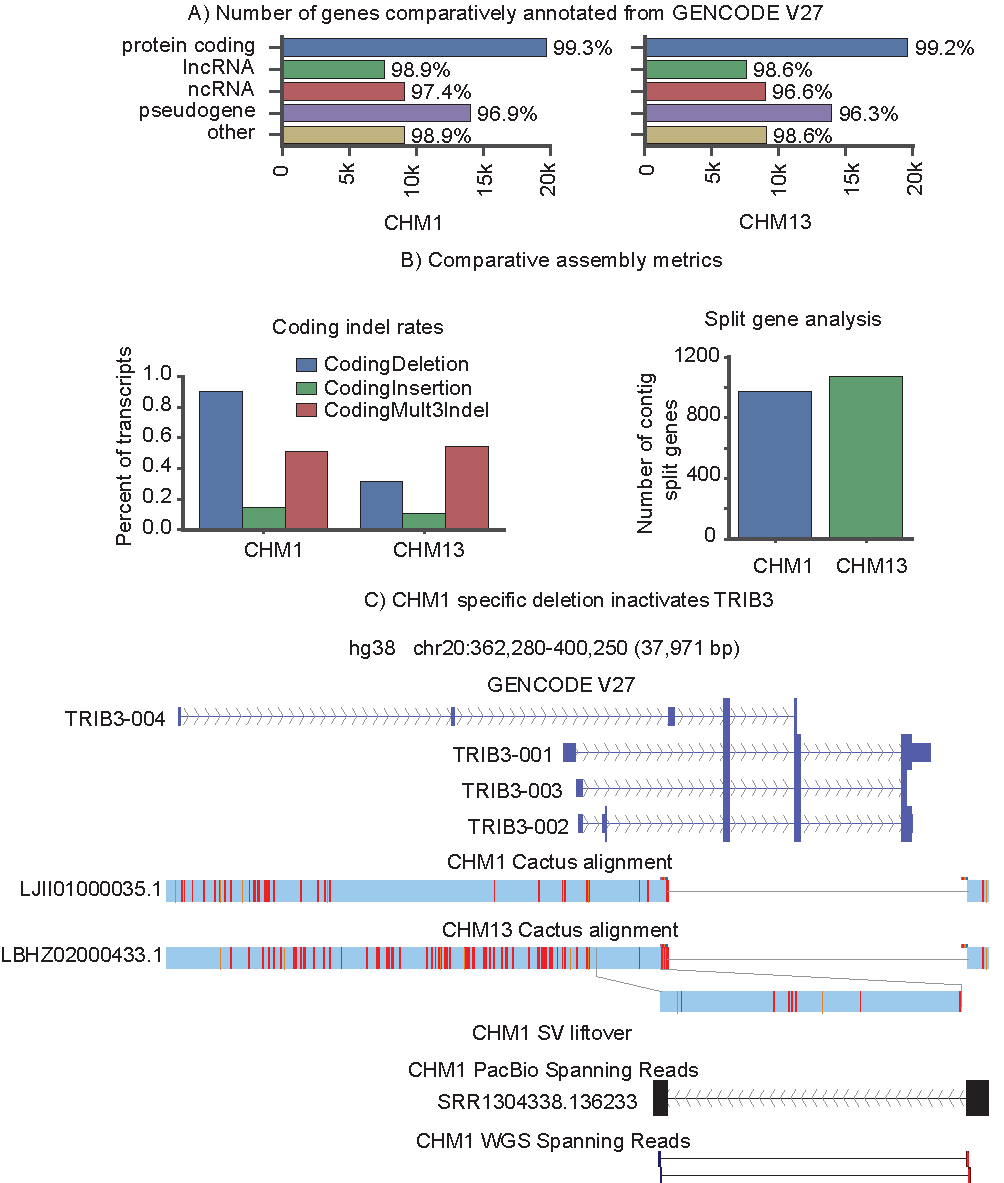
\includegraphics[width=\textwidth,height=0.7\textheight,keepaspectratio]{figure3-human-v2.pdf}
\caption{Pseudo-diploid human annotation}
A) The number of genes comparatively annotated from GENCODE V27 onto each assembly are reported. Percentages are the percent of GENCODE V27 this number represents. GENCODE biotypes are simplified into protein coding, lncRNA, ncRNA, pseudogene and other. Other includes processed transcripts, nonsense-mediated decay, and immune-related genes. B) Comparative assembly metrics diagnose assembly quality. Frame shifting insertions, deletions and multiple of 3 indels that do not shift frame are reported for each assembly (left). Consistent with the great ape genomes, there is a systematic over-representation of coding deletions, despite these assemblies coming from haploid cell lines. Split gene analysis reports on how often paralog-resolved transcript projections end up on different contigs, which can diagnose assembly contiguity. C) Analysis of genes found in one genome and not the other led to the discovery of a novel structural variant specific to CHM1, which disables the gene TRIB3. Spanning reads were found in both PacBio and Illumina whole genome sequencing that validate the deletion.
\label{fig:fig3}
\end{figure}

\begin{figure}
\centering
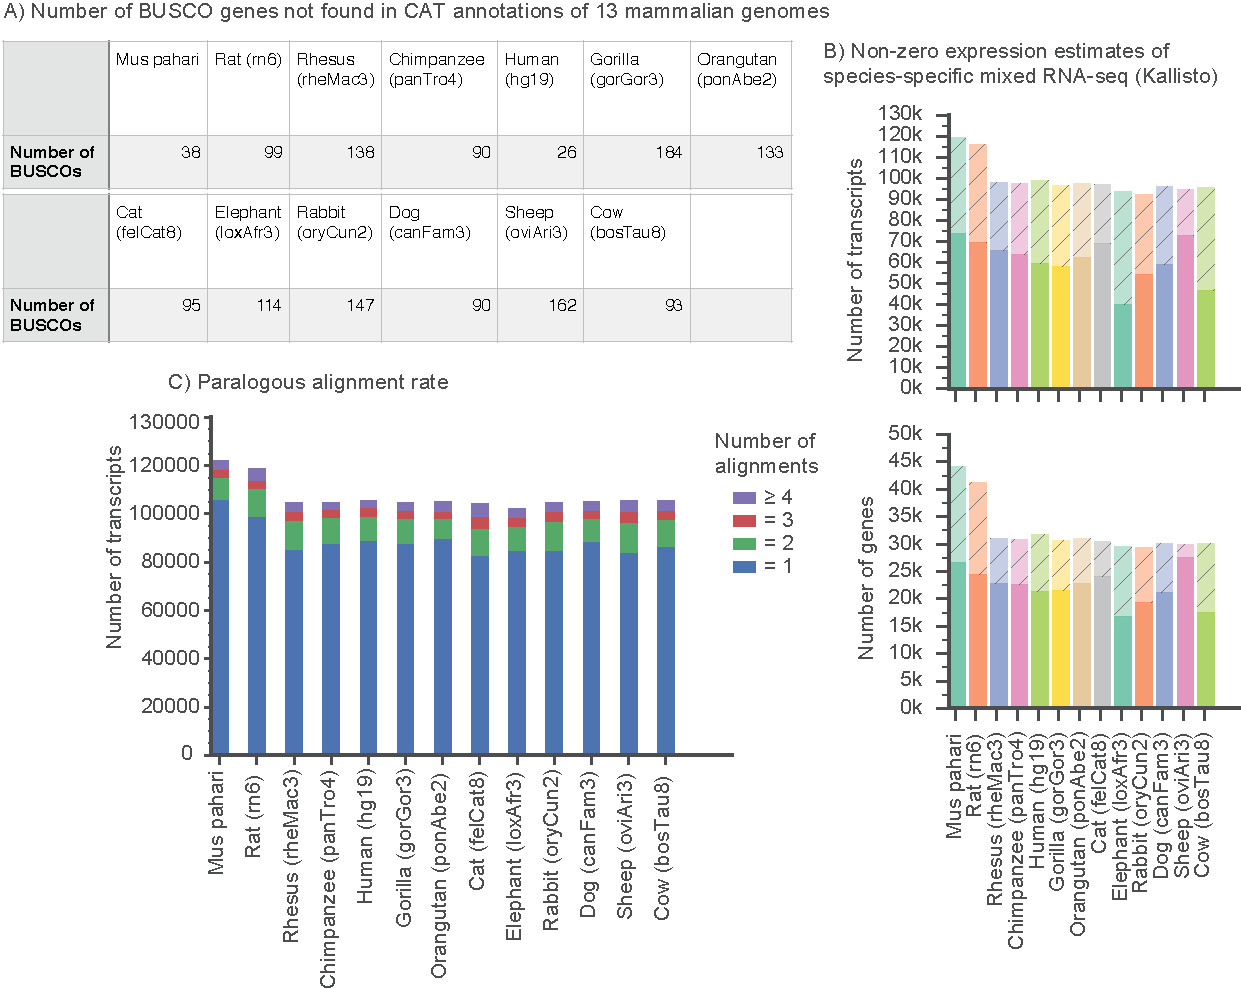
\includegraphics[width=\textwidth,height=\textheight,keepaspectratio]{13way.pdf}
\caption{14-way annotation}
A) BUSCO analysis of the annotation sets provides a benchmark for the completeness of the annotation sets. An average of 2.63\% of BUSCO genes are missing in the CAT annotation sets. B) The gene annotation sets for each of the 13 mammalian genomes were quantified against the mixed input RNA-seq sets obtained from SRA. Genes or transcripts with TPM\textgreater 0.1 are solid colors, while genes or transcripts with no measurable expression are shaded. An average of 2.8  isoforms per gene per genome had quantifiable expression, suggesting that CAT can infer isoform information across long branch lengths. C) Paralogous alignments of protein coding genes are quantified in each of the 13 mammalian genomes. Paralogy is measured using a sliding window filter over transcript projections. The rate of paralogous alignments is relatively even across phylogenetic distance.
\label{fig:fig4}
\end{figure}

\begin{figure}
\centering
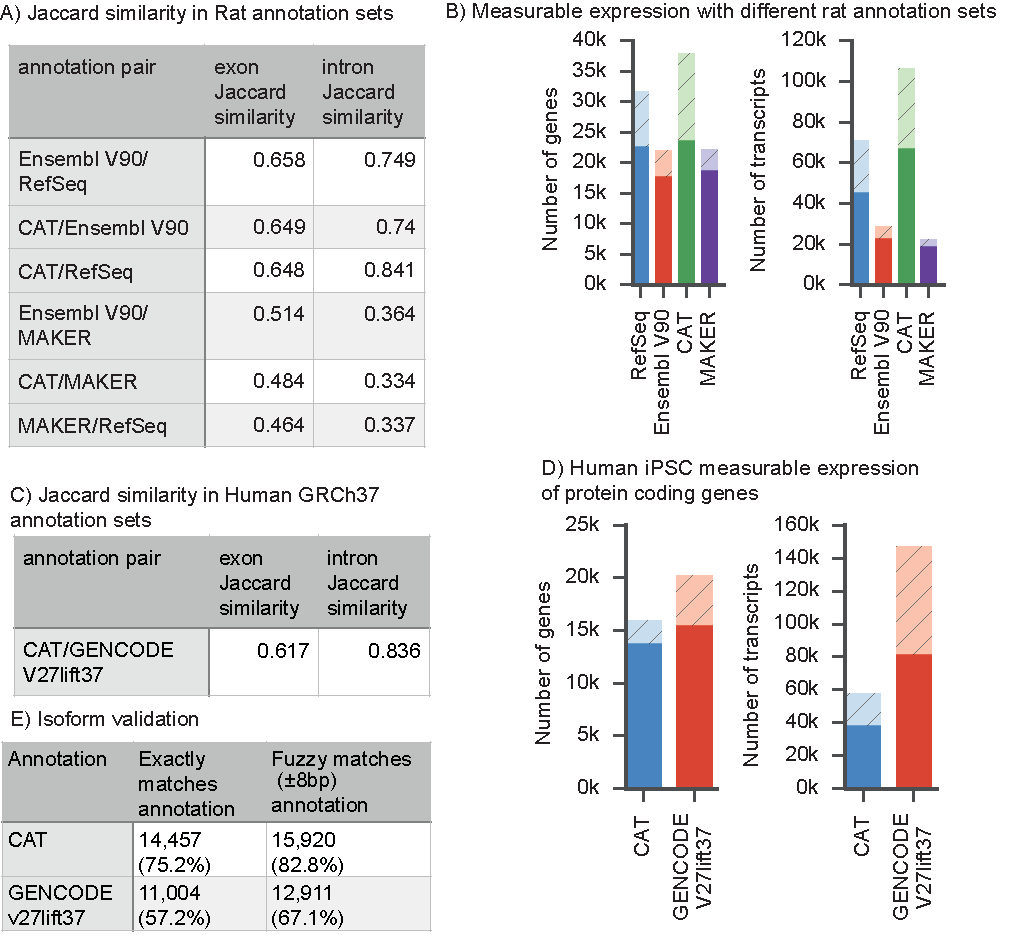
\includegraphics[width=\textwidth,height=\textheight,keepaspectratio]{figure5-rat_v15.pdf}
\caption{Validation of CAT annotation using rat and human}
A) Jaccard similarity of CDS introns and exons between rat annotation sets shows high similarity between CAT and Ensembl/RefSeq. B) Each transcript set was used to construct a Kallisto \cite{bray2015near} index, and then all of the input RNA-seq for annotation were quantified. Solid bars are genes or transcripts with non-zero expression (TPM \textgreater 0.1) estimates, while light hatched bars are transcripts or genes in the annotation set with zero expression. CAT provides an annotation set with slightly more detectable genes than other annotation methods, and far more detectable isoforms. C) Jaccard similarity of CDS introns and exons in human annotation sets. D) Kallisto measurable expression of human iPSC dataset against CAT protein coding annotation lifting mouse GENCODE VM15 to hg19 vs. GENCODE V27lift37. Even at large phylogenetic distance, CAT correctly annotates a comparable number of genes to a highly curated annotation set.
\label{fig:fig5}
\end{figure}

\clearpage
\beginsupplement

\section*{Supplementary text}
\section*{CAT pipeline detailed description}

Below is a walkthrough of the CAT pipeline. Please see the README on github ((\url{https://github.com/ComparativeGenomicsToolkit/Comparative-Annotation-Toolkit}) for the most up to date information as well as practical information on how to run the pipeline 

\subsection*{Whole genome alignment}
	CAT relies on a reference-free whole genome alignment produced by the tool progressiveCactus. One or more of the genomes in the alignment should be a high quality reference whose existing annotations will be projected. Care should be taken when generating cactus alignments to provide sufficient outgroup genomes. Having high quality outgroups improves the resolution of paralogies and rearrangements.

\subsection*{Alignment chaining}
	CAT converts HAL format alignments into pairwise genome alignments via a conversion to the UCSC chain format \cite{kent2003evolution}. This is accomplished by using the halLiftover tool to provide a PSL-format alignment describing each pairwise relationship to the high quality reference, and this alignment is then chained via the axtChain tool. 
    
\subsection*{transMap}
	transMap \cite{stanke2008using,zhu2007comparative} is a process for using pairwise whole genome alignments to project transcript annotations from one genome to another. The main program in the Kent repository for this process is pslMap. Custom software was written for CAT and included in the Kent repository, including pslMapPostChain which chains together mapped over transcript projection, and transMapPslToGenePred which converts the transcript projections to a gene model, keeping track of frame information and optionally filling in coding and non-coding gaps. Frameshifting gaps are not filled. CAT currently hard-codes those values at 50bp and 80bp respectively.
    
\subsubsection*{transMap filtering and paralogous alignment resolution}
	After transMap projection, alignments are filtered to their most likely ortholog, and paralogies are detected. This is performed using the tool pslCDnaFilter from the Kent repository in two parameterizations. The first parameterization does not actually filter the alignment set, but detects paralogies by relying on the localNearBest algorithm. This algorithm filters alignments based on windows of the input sequence. This process will keep multiple alignments for a given input sequence if they are in non-overlapping portions of the source transcript. This algorithm was originally designed for highly discontiguous assemblies. CAT leverages this concept to instead detect paralogies by looking at the difference. Alignments that localNearBest filter out are likely to be paralogous alignments and not instances of discontinuity, and so can be flagged as such. Putatively paralogous alignments are filtered further setting minSpan to 0.2 and providing a user-changeable minimum paralog coverage, which defaults to 50. minSpan is an effective filter against retroposed pseudogenes by filtering out any projection whose genomic size is smaller than 20\% of the source transcript. The minimum paralog coverage flag does not consider any alignments whose query coverage is smaller than that value as a paralog, providing extra filtering for discontinuity. The best localNearBest parameter depends on the phylogenetic distance and assembly qualities involved, and can require tuning. The default value in CAT is 0.2, which is a fairly relaxed value. Decreasing this value will increase the rate at which discontinuity is called as paralogy.
    
	The actual filtering of transMap projections is performed by the globalNearBest algorithm parameterized to 0, which forces pslCDnaFilter to pick the one highest scoring alignment for each input sequence. In this mode, the same minSpan value of 0.2 is used, and a minimum coverage of 10\% is required. After this step, a locus resolution step is performed to make sure that all transcripts from a given source gene end up in the same location. If globalNearBest ended up choosing multiple disjoint loci for a given gene, the highest average score locus is chosen and then lower scoring alignments for transcripts assigned elsewhere are chosen in this locus, if they exist.

\subsection*{AUGUSTUS}
	CAT runs the gene finding tool AUGUSTUS in up to four distinct parameterizations -- AugustusTM (TM), AugustusTMR (TMR), AugustusCGP (CGP) and AugsutusPB (PB). The output of each of these modes is combined with the original transMap output in the consensus gene set finding process. The first two modes, TM/TMR are intended to reproduce the input isoform exactly, fixing regions where the alignment dropped an exon or introduced a small gap, or where the splice site may have shifted. These modes cannot detect novel genes or transcripts. In contrast, CGP/PB both can detect novel isoforms and genes. However, CGP can only detect one isoform for a locus and cannot find UTRs. CGP also cannot find genes in regions that did not align. 
    
\subsubsection*{AugustusTM/AugustusTMR}
	The primary parameterization of AUGUSTUS for comparative annotation is primarily a method to clean up transMap projections. Due to a combination of assembly error, alignment noise and real biological changes transMap projections have frame shifting indels, missing or incomplete exons, and invalid splice sites. TM is given every protein coding transMap projection one at a time with some flanking sequence and asked to construct a transcript that closely matches the intron-exon structure that transMap provides. Since AUGUSTUS enforces a standard gene model, frame shifts and invalid splices will be adjusted to a valid form. In some cases this will mangle the transcript, producing either another isoform or something that does not resemble the source transcript. TMR runs the same genomic interval and also transMap derived hints through AUGUSTUS, but with less strict weights on the transMap hints and with the addition of extrinsic hints from RNA-seq and/or IsoSeq. This is particularly useful in regions where an exon was dropped in the Cactus alignment.
    
\subsubsection*{AugustusCGP}
	As TM/TMR is built on the transMap projections, it can neither identify novel genes nor existing genes of the reference annotation for which the mapping entirely failed. For this purpose, AUGUSTUS is run in its new comparative mode (CGP) recently published \cite{konig2015simultaneous}. This mode uses a novel objective function to simultaneously predict coding transcripts in every genome in a Cactus alignment, taking in extrinsic information from any provided existing annotations as well as RNA-seq and/or IsoSeq data in any of the aligned genomes. The genome alignment is used to exploit evolutionary content for gene finding (e.g. sequence conservation, conservation of exon boundaries and selective pressure) and to transfer extrinsic evidence across genomes. The latter has the effect that each genome can benefit from the combined evidence for the clade. CGP performs best when high quality RNA-seq derived from polyA selected libraries is provided for as many genomes as possible. If this is not available, consider providing a FASTA file with previously annotated proteins of one of the currently annotated genomes. 
    
\subsubsection*{AugustusPB}
	PB is run when IsoSeq data are provided and the appropriate flags set. PB runs AUGUSTUS in single genome \textit{ab-initio} + evidence-based gene finding mode, providing high weight to extrinsic hints derived from IsoSeq data, and with the model parameterized to allow for alternative isoforms. PB provides the advantage of being able to detect genes in regions that did not align to any of the other genomes.
    
\subsubsection*{Parent gene assignment}
CGP/PB transcripts are then assigned a possible source transcript by comparing their genomic overlap with both filtered and unfiltered transMap projections. If a transcript is assigned to an orthologous projection, then it will be evaluated for being a novel isoform during consensus finding. If a transcript is assigned to a projection that was filtered out during paralog resolution, then it is a candidate being a possible paralog. A likely cause of this situation is a gene family expansion. If a transcript does not overlap with any transMap projections, then it is a candidate novel gene. However, the false positive rate of these is inherently high due to the likelihood of novel genes being dwarfed by the likelihood of assembly or alignment errors leading to no transMap projections in the region.

\subsubsection*{Transcript classification}
	transMap projections are classified by a series of classifiers that evaluate their strength. These classifiers include evaluating whether the projection was complete (100\% coverage), alignment identity, whether the projection ran off the edge of a contig, whether the projection had a 1-1 ortholog relationship, and importantly how many of the exon junctions lie nearby in transcript coordinate space. This original intron classification is very important when assigning isoform relationships. Due to alignment errors and real biological changes, transMap projections may have gaps that are not near the source transcript exon junctions. The number of original introns is an important feature in the consensus finding process, protecting from retroposed pseudogenes as well as isoform switching.
    
	Transcripts produced by TM/TMR are also classified. To do so, they are first aligned in transcript space using BLAT \cite{kent2002blat}. Alignments are performed twice, once on a whole transcript mRNA level and once using the in-frame CDS sequence using a mode of BLAT that does translation alignment. The mRNA alignments are used to perform the same original intron analysis described above, as well as record standard alignment metrics such as coverage and identity. The CDS alignments are used to evaluate transcripts for having frame shifting indels. A track of the frame shifting indels are added to the assembly hubs produced.

\subsubsection*{homGeneMapping}
	homGeneMapping is a tool in the Augustus package for cross-species evaluation of gene sets. It uses Cactus alignments to project the coordinates of genomic features to other genomes. Homologous gene structures are evaluated based on their consistency across species and their agreement with the combined extrinsic evidence for the clade. The latter effectively means, that a gene structure of a species with no native evidence can be "confirmed" with evidence for another species by mapping it through the genome alignment. CAT uses homGeneMapping to evaluate intron and exon features in the target genomes for 1.) consistency with the reference annotation and 2.) having extrinsic support by the combined RNA-seq and/or IsoSeq. These measures of support are used in the consensus finding process.

\subsubsection*{Consensus finding}
	The consensus finding process takes in transcripts from every mode and attempts to find the highest quality ortholog for a source transcript. The modes that are capable of predicting new transcripts are also evaluated for providing novel isoforms or novel loci. The final gene set is output with a series of features measuring how confident the prediction is.
    
	To evaluate transMap, TM and TMR transcripts a consensus score is assigned to each. This score is the sum of the alignment identity target alignment coverage, intron/exon annotation support, original intron support, and intron/exon RNA-seq/IsoSeq support if extrinsic data were provided.
    
	If CGP and/or PB is run, then the those transcripts are evaluated for providing novel information. If a prediction did not overlap any transMap projections, then it is tagged as putative novel and incorporated into the gene set. If a prediction overlaps a transMap projection that was filtered out during paralog resolution, then it is tagged as a possible paralog as well as with the names of overlapping transcripts and incorporated into the gene set. If a prediction overlaps a transMap projection and contains a splice junction not seen in the reference annotation, then it is tagged as a novel isoform and incorporated into the gene set as a member of the gene it overlapped with.
    
	After consensus finding is complete, a final filtering process is performed. This filtering process deduplicates and strand resolves the transcript set. Duplicates most often occur when the AUGUSTUS execution modes create an identical transcript model from different input isoforms. In this case, the duplicates are removed and the remaining transcript tagged with the names of alternative source transcripts. Finally, strand resolution throws out transcripts that are on opposite strands. The correct strand is chosen by looking at which contains the most high quality transcripts.
    
	The consensus finding process provides many user-tunable flags that can be adjusted based on the phylogenetic distances being considered. Users can change how many exons and introns should be supported by the reference annotation and extrinsic sources before being considered. Users can also decide if they want only to consider extrinsic data within that individual species or within all species in the alignment. 

Another consideration is the quality of the input extrinsic data. Low quality RNA-seq data, or RNA-seq libraries not polyA selected, lead to a higher false positive rate in CGP. These often manifest as small single exon transcripts that can inflate the rate of putative novel gene calls. Adjusting a cutoff for the number of exons required to be considered novel can help drill down to a set of interesting candidates.

\clearpage

\begin{figure}
\centering
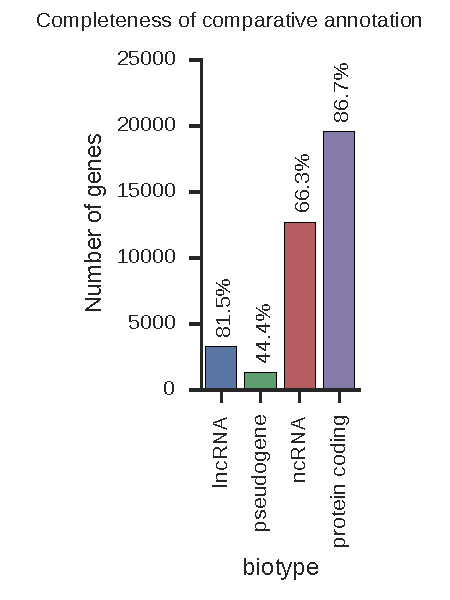
\includegraphics[]{rat_completeness.pdf}
\caption{Rat completeness}
The number of genes comparatively identified in the rn6 assembly from mm10 GENCODE VM11, broken down by simplified biotypes. The percentages on top are the percent of the total genes in each simplified biotype present in VM11. While a large portion of protein coding genes are identified, much fewer lncRNAs and other non-coding biotypes are identified.
\label{supp_fig:rat_completeness}
\end{figure}


\begin{figure}
\centering

A)

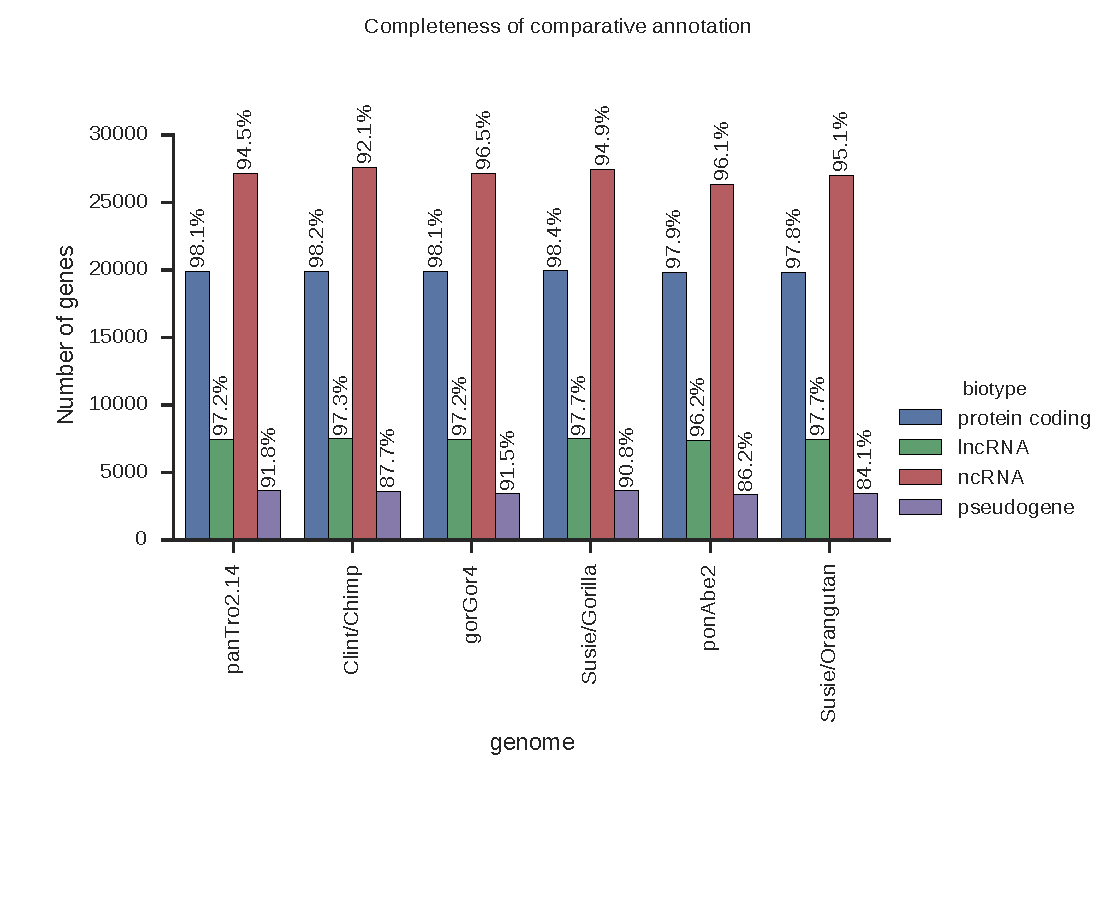
\includegraphics[scale=0.7]{primate_completeness_old_and_new.pdf}

B)

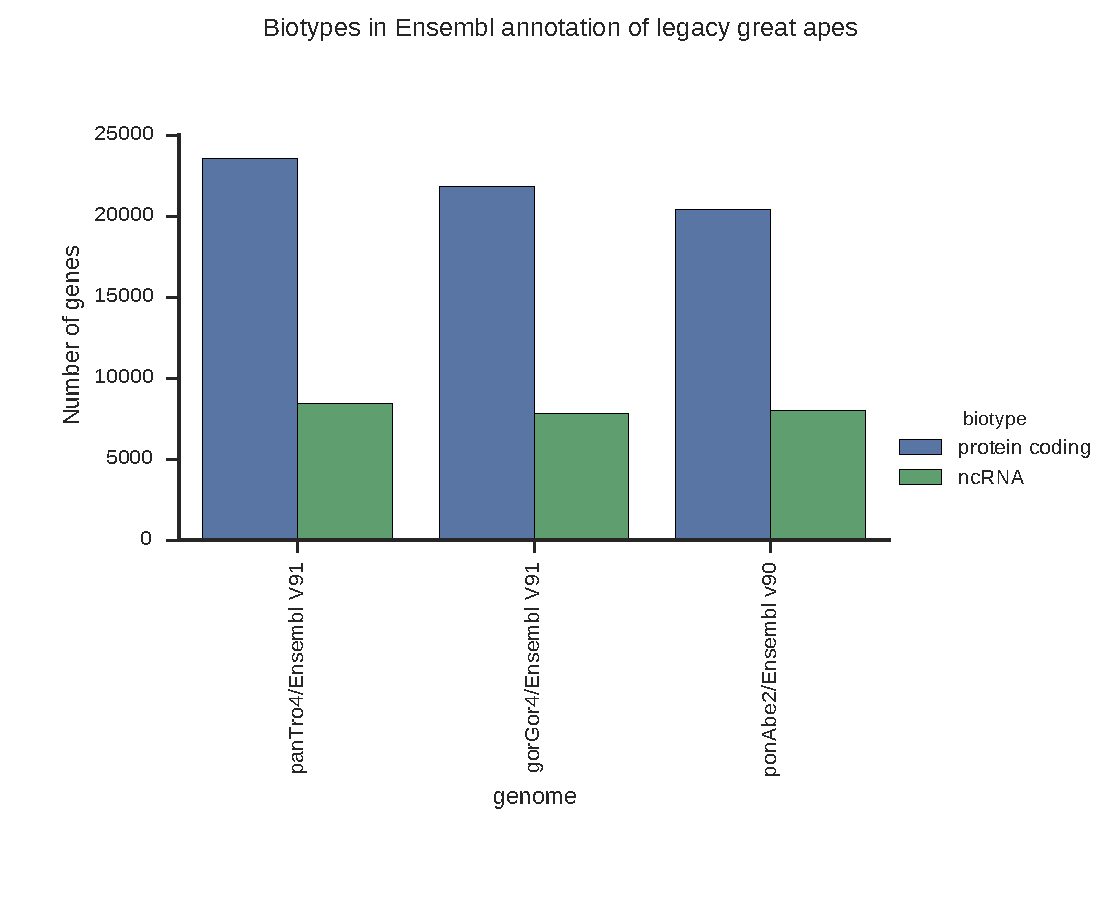
\includegraphics[scale=0.5]{ensembl_primate_biotypes.pdf}

\caption{Primate completeness and biotypes}
A) Percent of genes in simplified biotypes identified in both generations of great ape assemblies. The numbers above the bars are the percent of GENCODE V27 genes identified broken down by simplified biotypes. The number of genes identified in the PacBio assemblies increased slightly for all of the great apes. B) The biotypes of the Ensembl annotations for the legacy great apes. Compared to the 19,836 protein coding genes in GENCODE V27, these annotation sets have 23,534, 21,795 and 20,424 protein coding genes for chimpanzee, gorilla and orangutan respectively, suggesting misclassified non-coding loci. We found 940 loci in chimp, 1,728 loci in gorilla and 1,270 loci in orangutan which are labeled as protein coding in Ensembl but are labeled other biotypes in the CAT annotation. Not only does CAT make tracking orthology relationships easier, but it also provides much higher correlation with real data, greatly improving cross-species RNA-seq analysis.
\label{supp_fig:primate_completeness}
\end{figure}

\begin{figure}
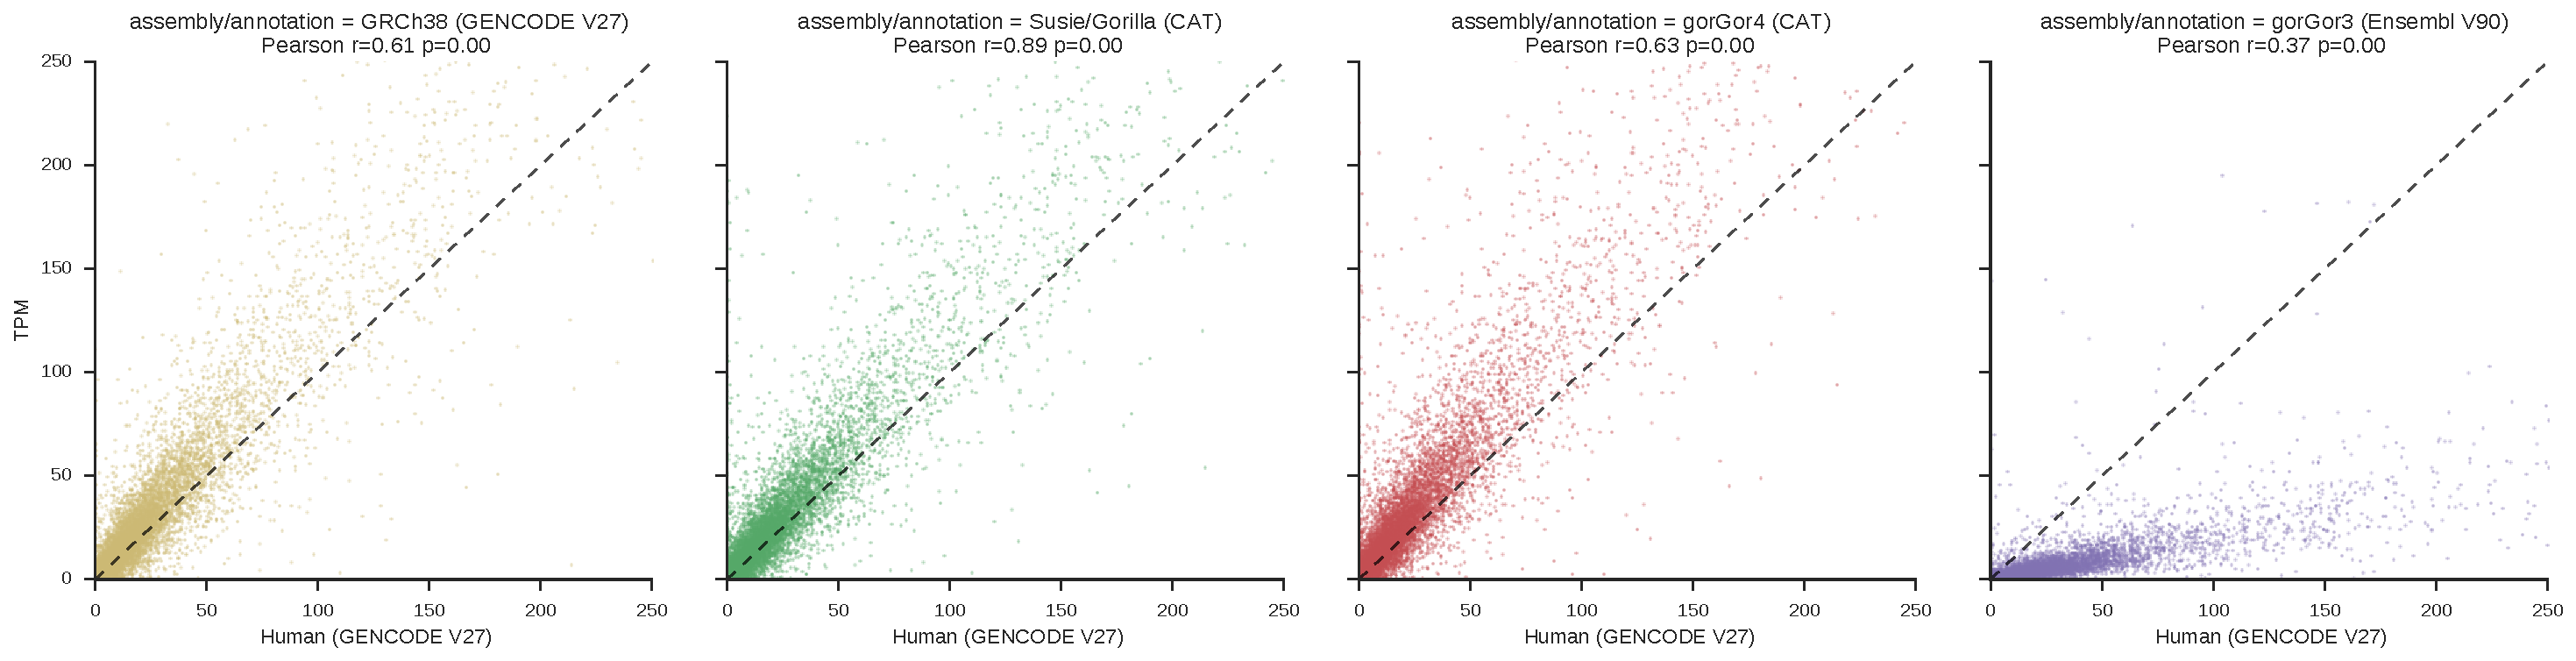
\includegraphics[width=0.8\paperwidth,keepaspectratio]{gorilla_kallisto.pdf}

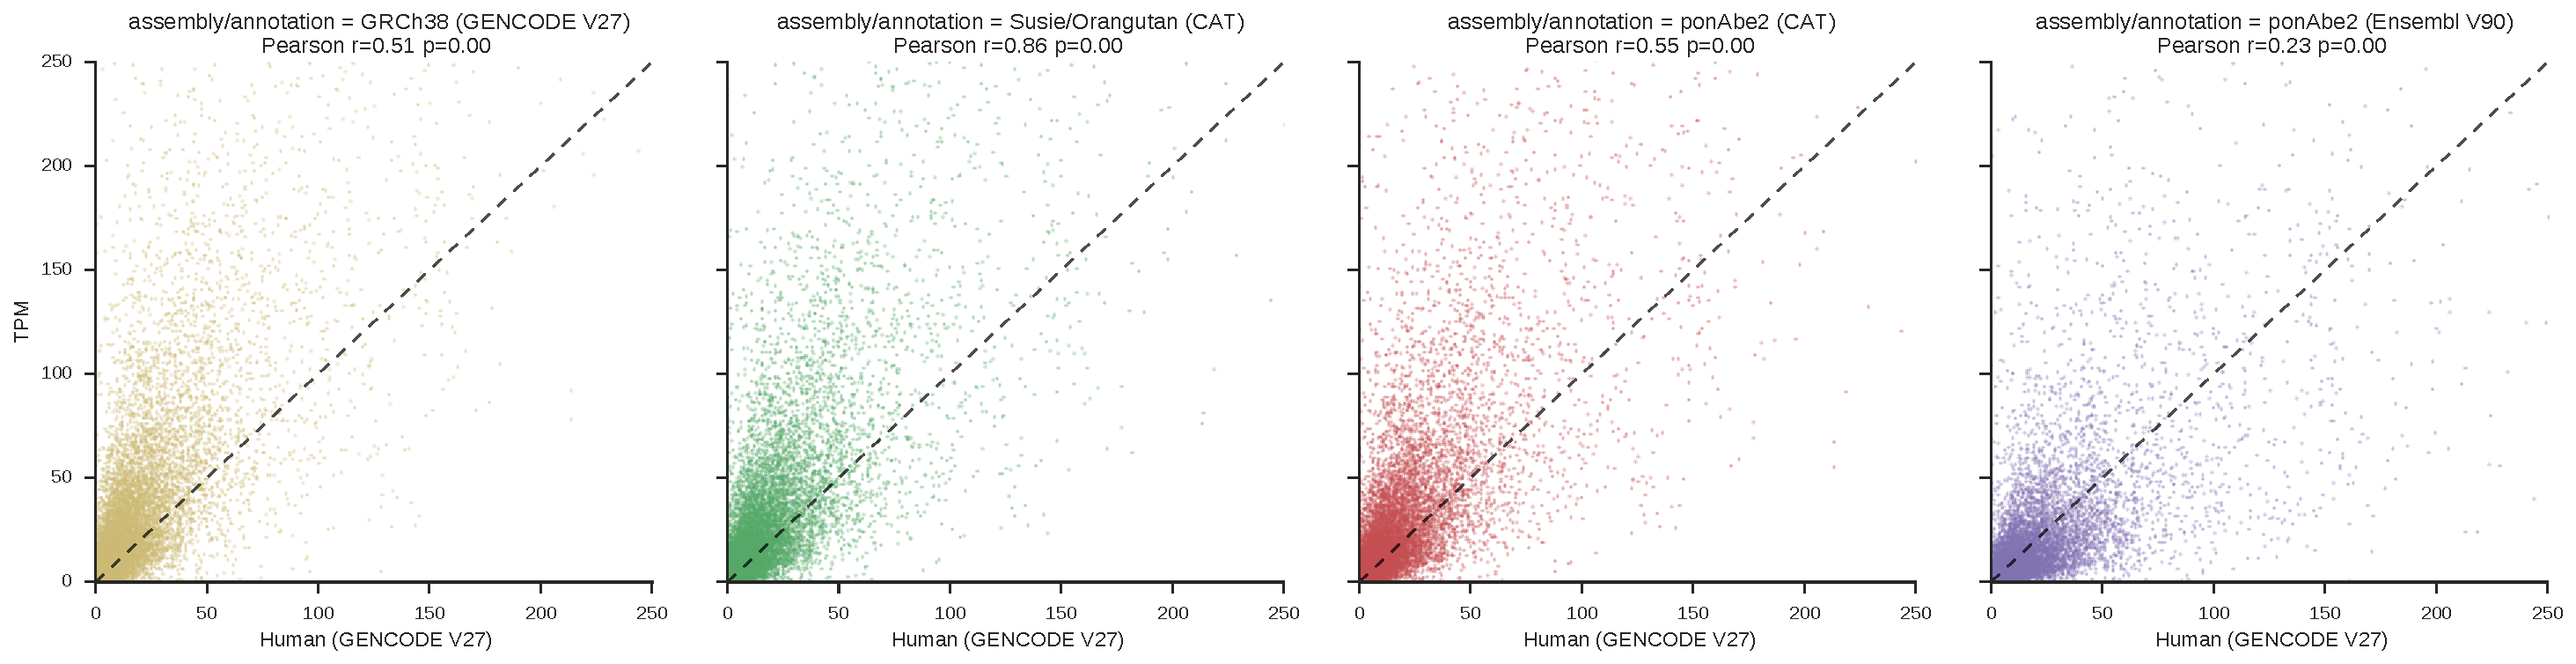
\includegraphics[width=0.8\paperwidth,keepaspectratio]{orangutan_kallisto.pdf}
\caption{Cross-species RNA-seq expression estimates}

Gorilla and orangutan iPSC RNA-seq are compared to human iPSC RNA-seq using a variety of annotation and assembly combinations. All comparisons were performed with Kallisto. Cross-species comparison was used by tracking gene common names. Because the pre-release of Ensembl V91 provided to us lacked common names, we used V90. Ensembl V90 annotation is on gorGor3, so that genome was used. The x-axis in all plots are the TPM of human iPSC data mapped to GENCODE V27. The y-axis in all plots is the TPM of species-specific iPSC RNA-seq mapped to the assembly/annotation pair in the title. These comparisons are filtered for protein coding genes, and In all cases, using the newest version of the assemblies with CAT provides the highest correlation.
\label{supp_fig:primate_expression}
\end{figure}

\begin{figure}
\centering
A)
\makebox[\textwidth]{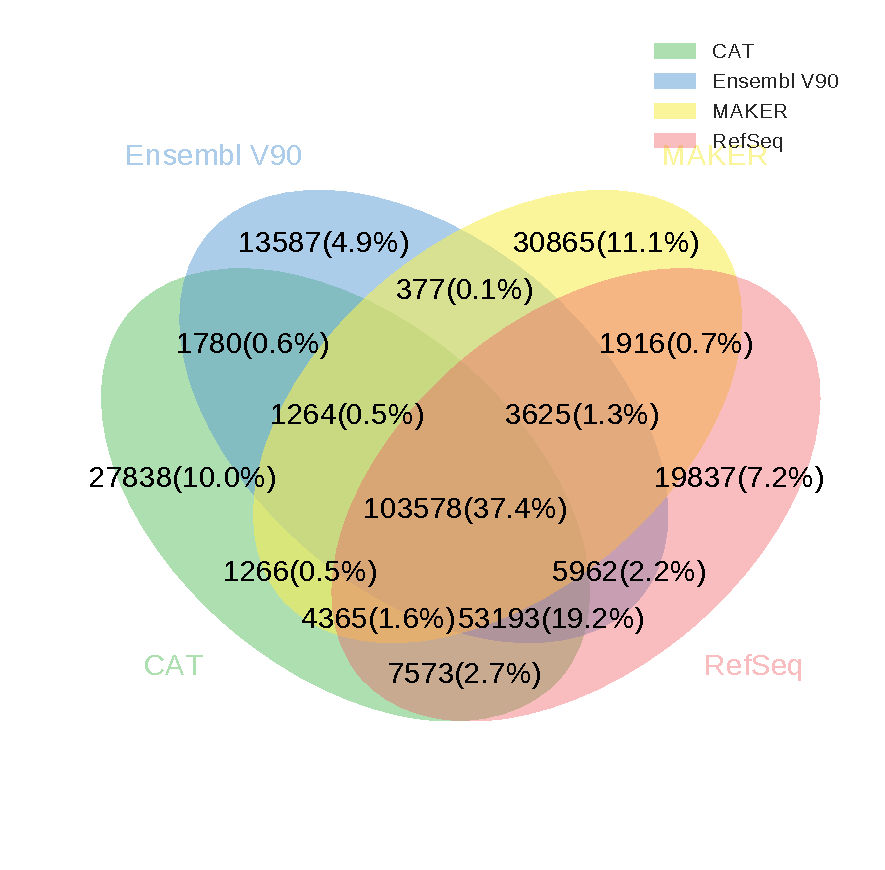
\includegraphics[width=0.45\paperwidth]{cds_intron_venn.pdf}}
B)
\makebox[\textwidth]{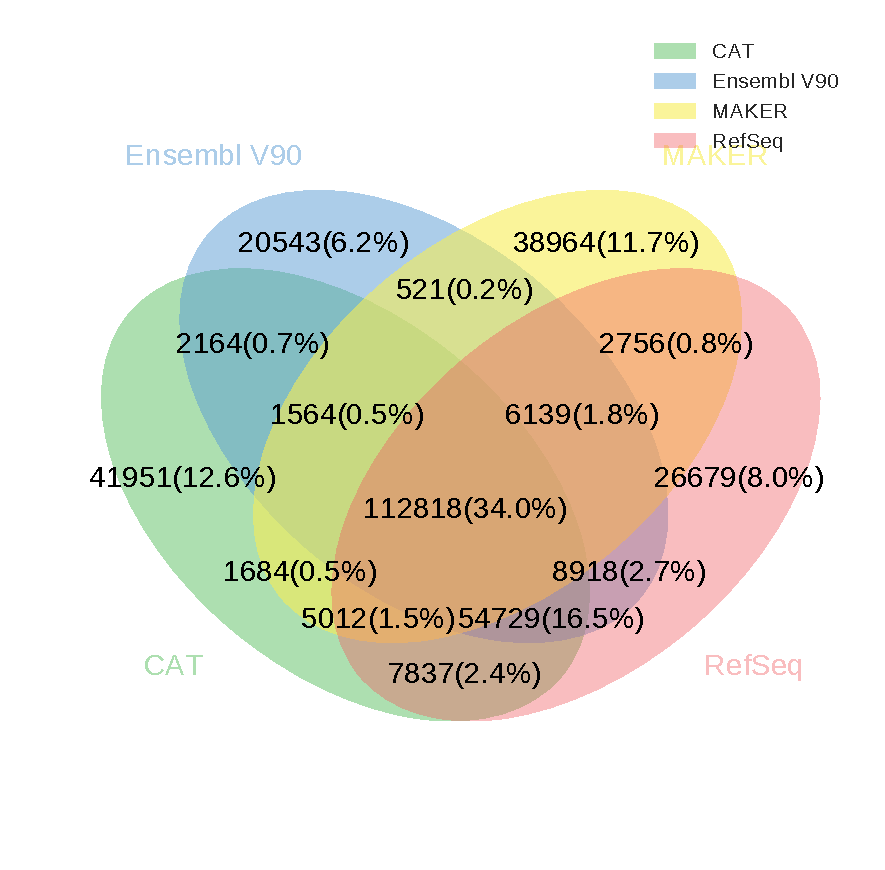
\includegraphics[width=0.45\paperwidth]{cds_exon_venn.pdf}}
\caption{Rat Exon/Intron Support Venn Diagram}
CDS Intron (left) and CDS exon (right) interval exact matches were compared between CAT, Ensembl V90, MAKER and RefSeq on rat rn6. MAKER had the highest proportion of unsupported exons and introns, followed by CAT. Only 37.0\% and 34.0\% of introns and exons respectively are present in all four annotation sets.
\label{supp_fig:rat_exon_intron}
\end{figure}

\begin{figure}
\centering
\makebox[\textwidth]{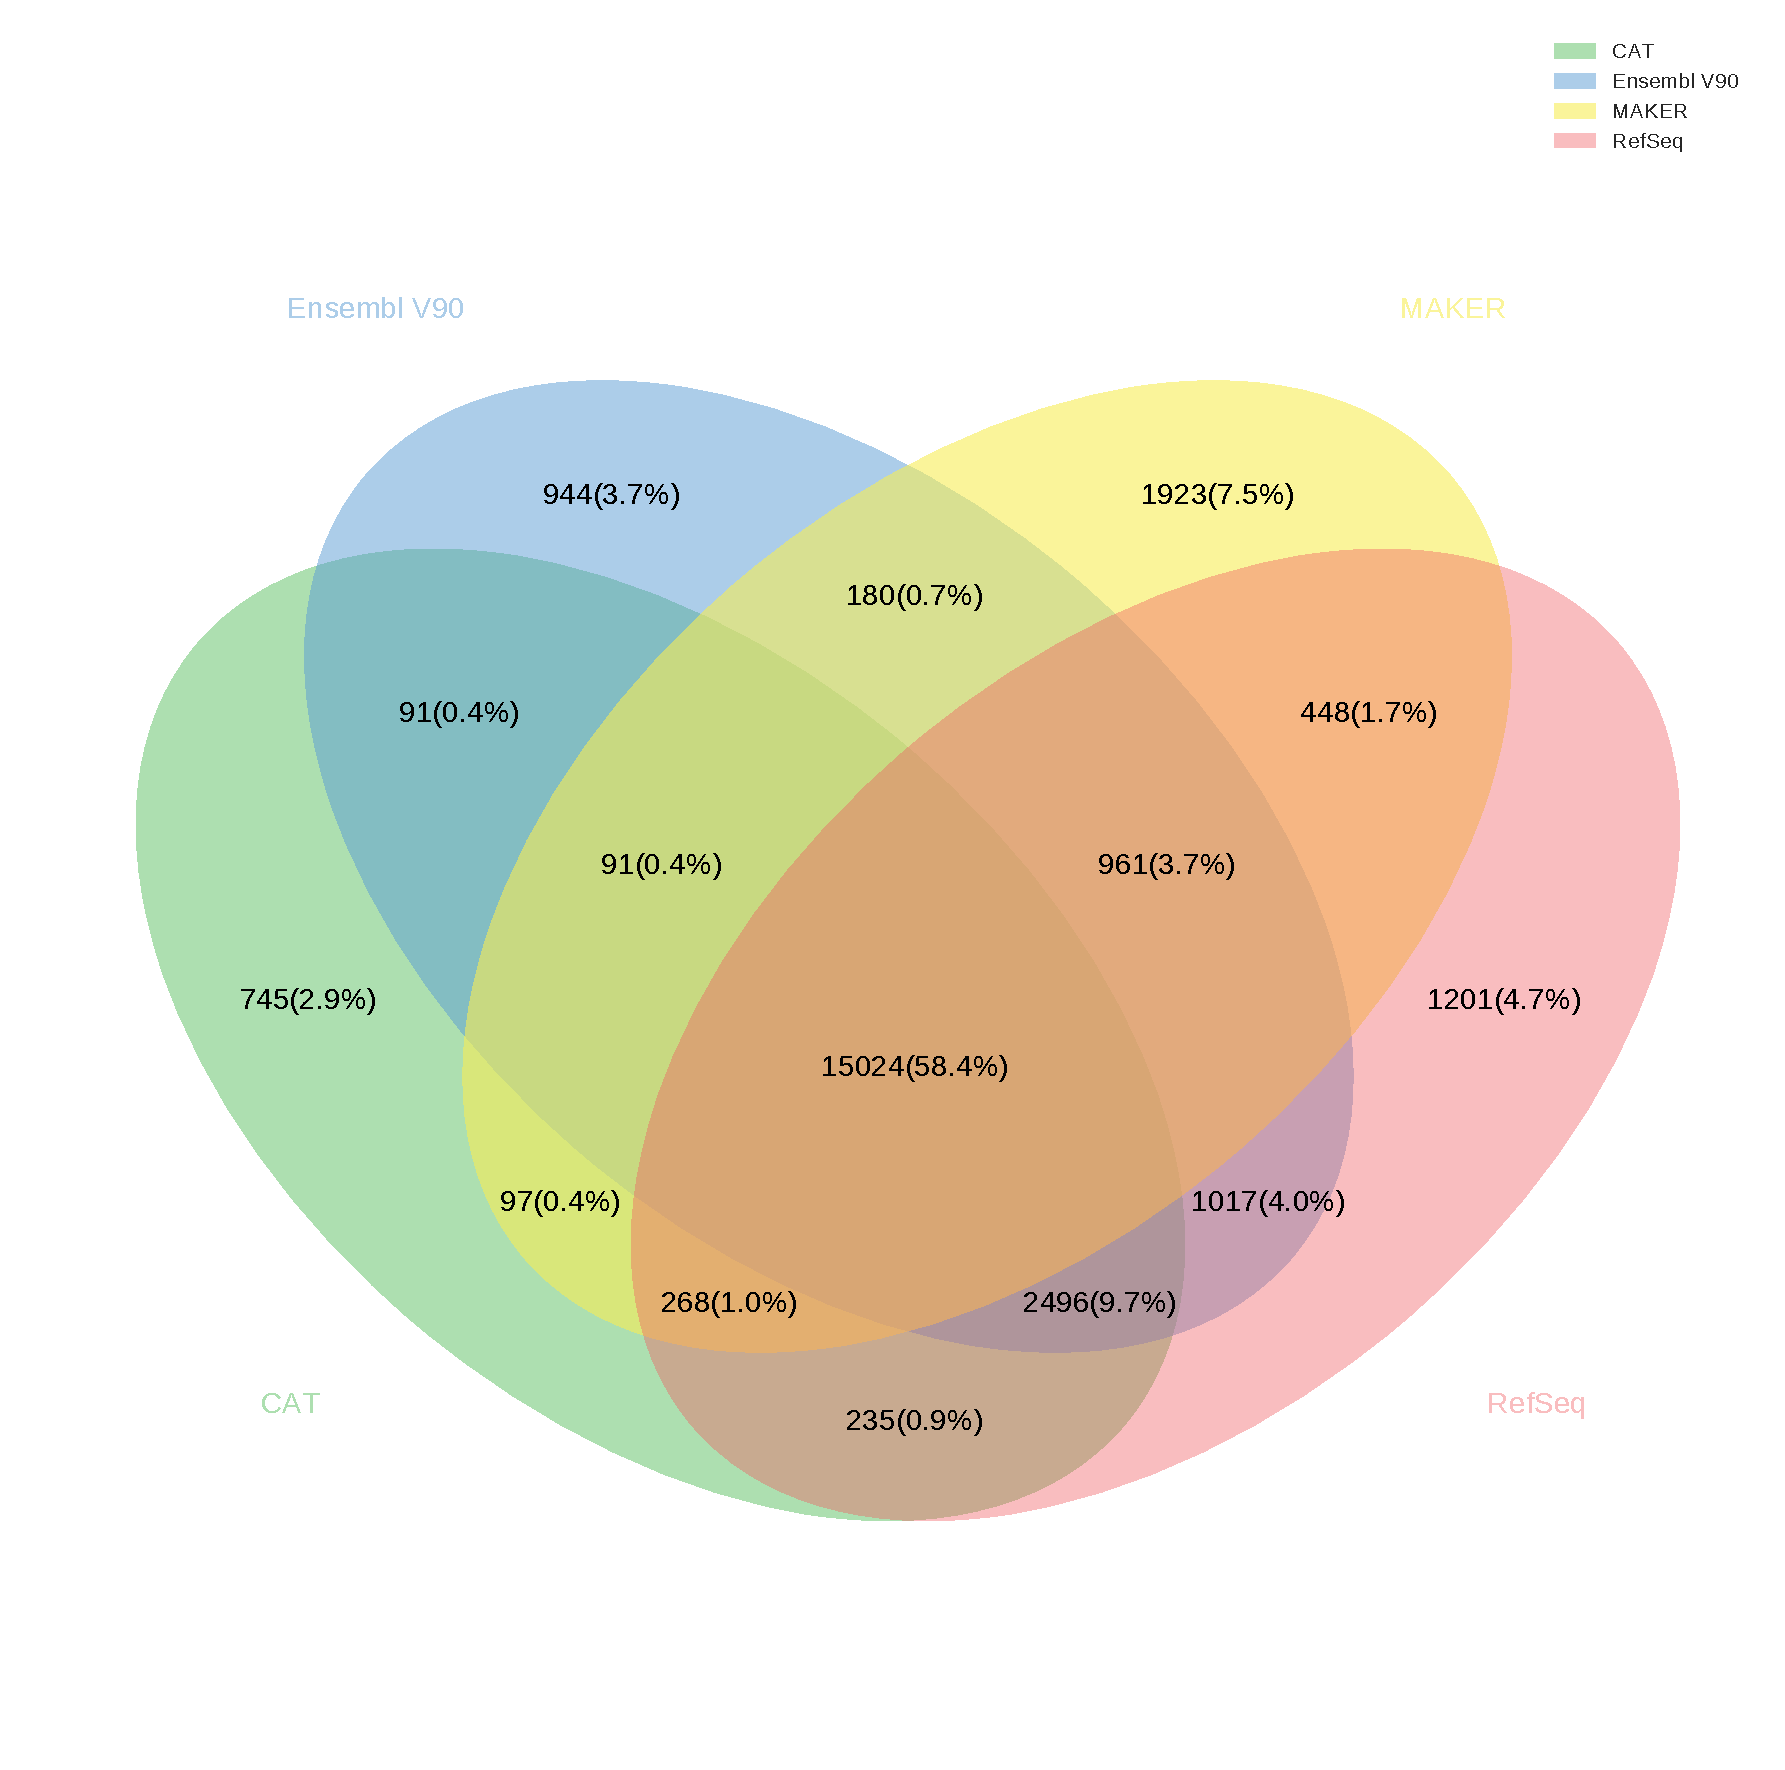
\includegraphics[width=0.8\paperwidth]{transcript_clusters.pdf}}
\caption{Rat Locus Venn Diagram}
Gene loci were compared between CAT, Ensembl V90, MAKER and RefSeq on rat rn6. Loci were clustered using the Kent tool clusterGenes, which requires exonic overlap on the same strand. Only 15,179 loci are shared between all sets.
\label{supp_fig:rat_locus_venn}
\end{figure}

\begin{figure}
\centering
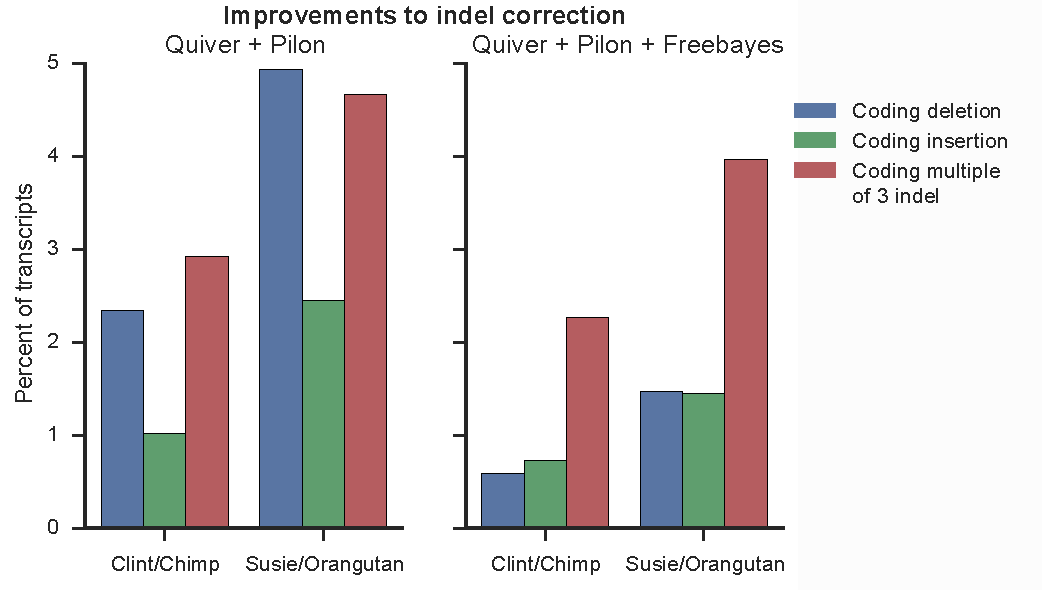
\includegraphics[width=\textwidth,height=\textheight,keepaspectratio]{primate_indels.pdf}
\caption{Primate Coding Indels}
The rate of transcripts with coding indels seen in the consensus gene sets for the SMRT primate assemblies are shown with Quiver and Pilon correction (left), and subsequent Freebayes \cite{garrison2012haplotype} based correction (right). Freebayes correction was not performed on GSMRT5 (gorilla). Coding indels are measured by pairwise translated BLAT alignments of a transcript to its ortholog in human. SMRT assemblies show a systematic over-representation of coding insertions. After Freebayes correction, the rate of insertions to deletions is roughly equal and lower than the rate of multiple of 3 indels, which is the expected result due to purifying selection.
\label{supp_fig:primate_indels}
\end{figure}

\begin{figure}
\centering
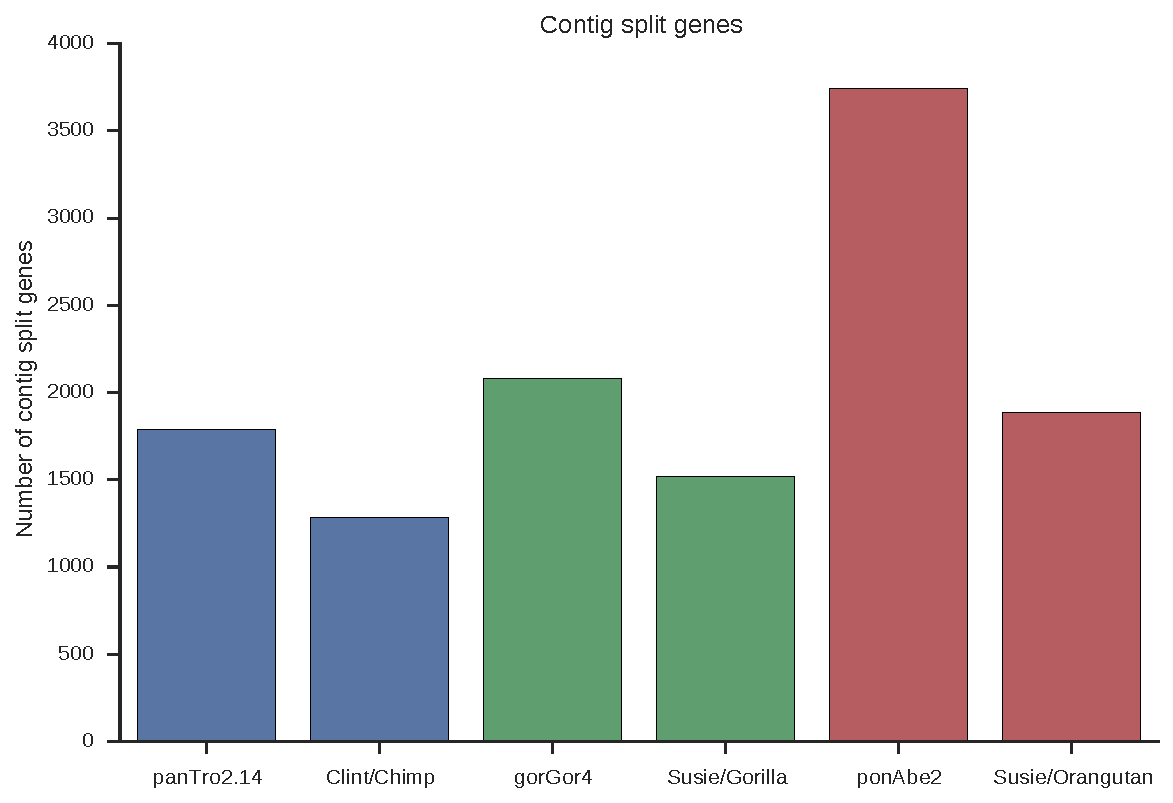
\includegraphics[width=\textwidth,height=\textheight,keepaspectratio]{split_genes.pdf}
\caption{Primate Split Genes}
\label{supp_fig:primate_split_genes}
Split gene analysis looks for transcript projections after paralog resolution that map to multiple contigs. This provides a metric for assembly contiguity. Despite the PacBio assemblies not being in chromosome sized pieces, fewer split genes are detected, suggesting that most contig breaks are not in genic regions.
\end{figure}

\begin{figure}
\centering
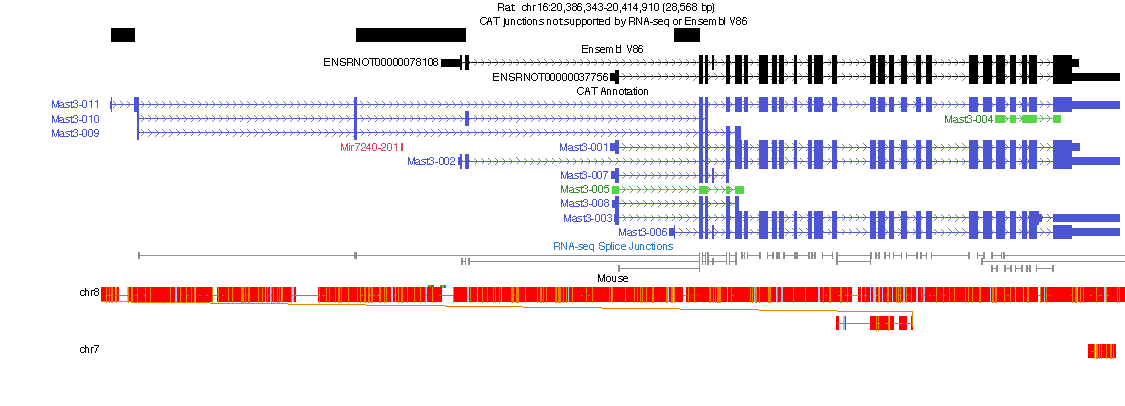
\includegraphics[width=\textwidth,height=\textheight,keepaspectratio,angle=90]{mast3_example.pdf}
\caption{Unsupported junctions example}
The rat gene Mast3 has two annotated isoforms in Ensembl supported by RNA-seq. CAT annotation added 9 new isoforms, two of which had unsupported junctions. These new annotations reveal an upstream transcription initiation site supported by RNA-seq. 
\label{supp_fig:unsupported_junctions}
\end{figure}

\begin{figure}
\centering
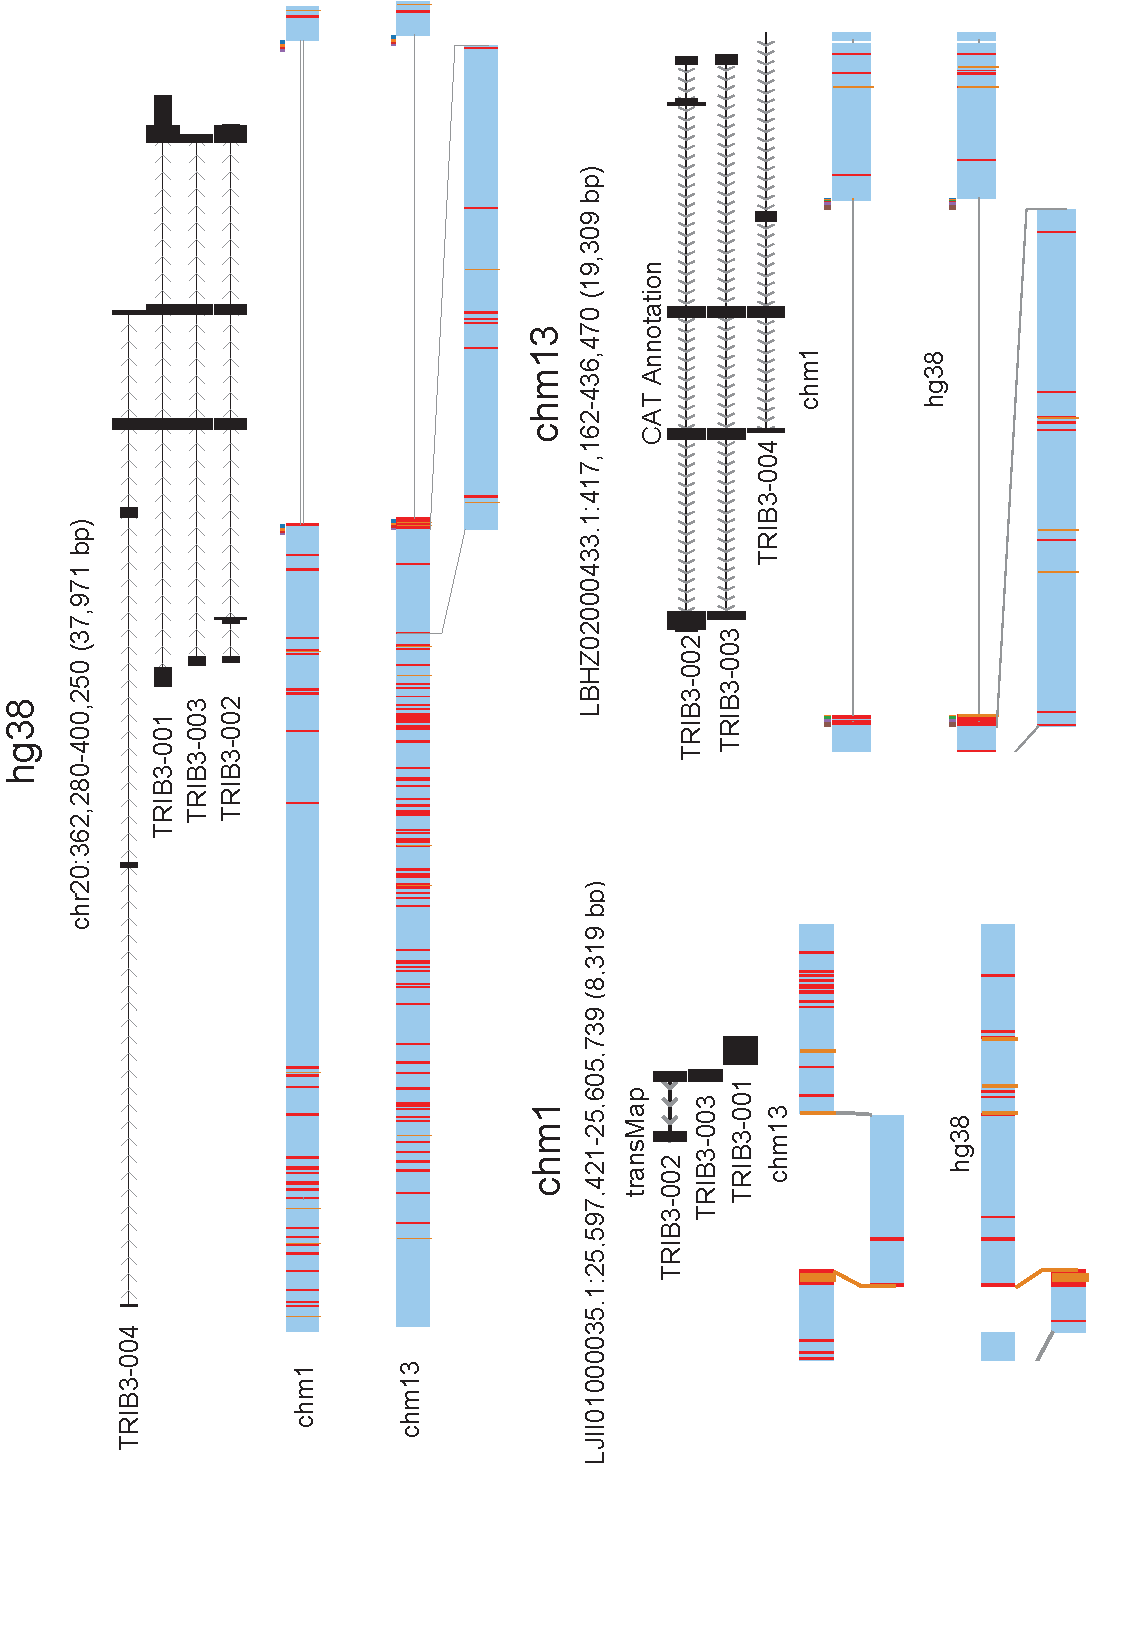
\includegraphics[width=0.8\textwidth,height=0.7\textheight,keepaspectratio]{trib3_full.pdf}
\caption{TRIB3 example}
The CHM1 structural variant in figure 4 is shown here from all perspectives. In CHM1, the short transMaps for the few remaining exons are filtered out and do not end up in the annotation set. In contrast, CAT annotated 3/4 of the isoforms. This figure shows the power of the UCSC assembly hub for evaluating structural variants by being able to view the alignment from any species present.
\label{supp_fig:trib3}
\end{figure}

\begin{figure}
\centering
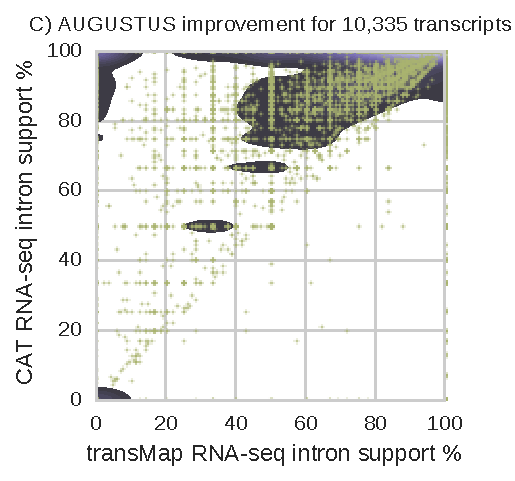
\includegraphics[width=\textwidth,height=\textheight,keepaspectratio]{augustus_rna_improvement_density_shade.pdf}
\caption{Rat AUGUSTUS improvement}
In consensus finding, 10,335 multi-exon protein coding transcripts were selected from one of the AUGUSTUS modes over the input transMap projection. One feature used for consensus finding is the relative RNA-seq support for intron junctions between transcripts, shown here. 
\label{supp_fig:augustus_rna_rat}
\end{figure}

\begin{figure}
\centering
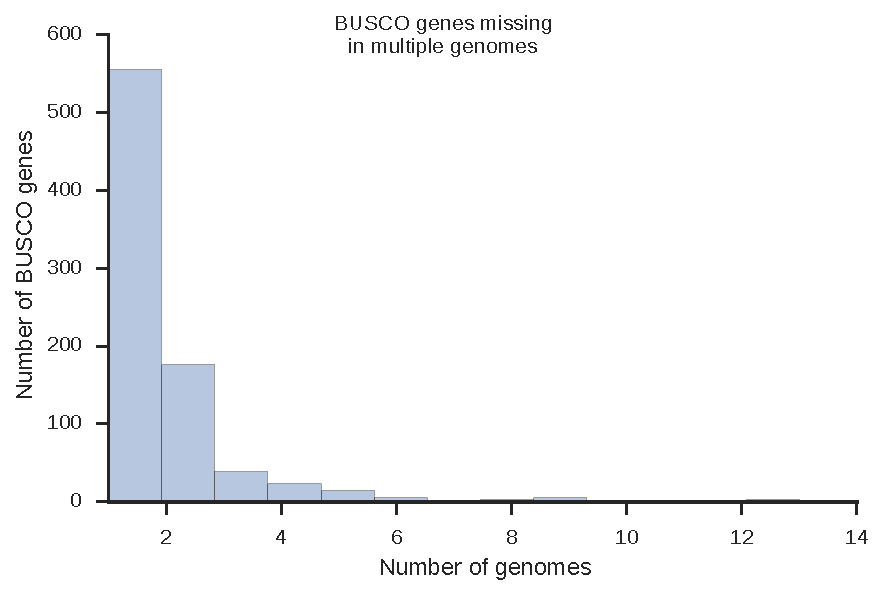
\includegraphics[]{busco_missing.pdf}
\caption{BUSCO genes missing in multiple genomes}
BUSCO analysis of the 13 mammalian genomes revealed very few missing genes are shared between genomes, suggesting that missing genes are related more to assembly completeness and alignment quality than a systematic bias in the annotation set.
\label{supp_fig:busco_missing}
\end{figure}

\begin{center}
\small
\captionof{table}{SRA RNA-seq accessions}
\label{supp_table:rnaseq_sra_table}
\begin{longtable}{|p{0.15\textwidth}|p{0.65\textwidth}|p{0.2\textwidth}|} \hline
Species   & SRA Accessions & Tissues \\ \hline
Rat       & SRR1041777, SRR1768421, SRR1768443, SRR1768444, SRR299123, SRR636875, SRR636876, SRR636877, SRR636925, SRR636926, SRR636927, SRR636970, SRR636971, SRR636972                                                                                                                                                                                                                                                                                   & Mixed, testis, liver, kidney, brain                                                                                   \\ \hline
Orangutan & SRR306792, SRR2176206, SRR2176207                                                                                                                                                                                                                                                                                                                                                                                                              & Brain, testis                                                                                                         \\ \hline
Gorilla   & SRR832925, SRR3053573, SRR306809, SRR306803, SRR306804, SRR306801, SRR306807, SRR306810, SRR306805, SRR306806, SRR306802, SRR306800, SRR306808                                                                                                                                                                                                                                                                                                 & Brain, 20 tissue pool                                                                                                 \\ \hline
Chimp     & SRR2040584, SRR2040585, SRR2040586, SRR2040587, SRR2040588, SRR2040589, SRR2040590, SRR2040591, SRR3711187, SRR3711188, SRR873622, SRR873623, SRR873624, SRR873625                                                                                                                                                                                                                                                                             & brain, heart, liver, testis, 8 week old iPSC derived neurons, undifferentiated iPSC                                   \\ \hline
Rhesus    & SRR306784, SRR306786, SRR306785, SRR2040593, SRR306783, SRR306787, SRR306780, SRR306778, SRR306790, SRR2040595, SRR2040594, SRR2040592, SRR306788, SRR306782, SRR306789, SRR306777, SRR306779, SRR306781                                                                                                                                                                                                                                       &    Kidney, liver, heart, brain, testis                                                                                                                    \\ \hline
Human     & ERR579132, ERR579133, ERR579134, ERR579135, ERR579136, ERR579137, ERR579138, ERR579139, ERR579140, ERR579141, ERR579142, ERR579143, ERR579144, ERR579145, ERR579146, ERR579147, ERR579148, ERR579149, ERR579150, ERR579151, ERR579152, ERR579153, ERR579154, ERR579155                                                                                                                                                                         & Ovary, tonsil, fallopian tube, placenta, endometrium, rectum, skeletal muscle, liver, fat, colon, smooth muscle, lung \\ \hline
Sheep     & SRR1653601, SRR1561187, SRR1561150, SRR1265856, SRR1536790, SRR1561171, SRR1265854, SRR1561367, SRR1561365, SRR1653570, SRR1653598, SRR1653597, SRR1266019, SRR1265849, SRR1653600, SRR1656805, SRR1561366, SRR1653594, SRR1561196, SRR1265855, SRR1653596, SRR1536788, SRR1266022, SRR1561156, SRR1266018, SRR1561195, SRR1536770, SRR1266020                                                                                                 &     Liver, brain, blood                                                                                                                   \\ \hline
Cow       & SRR2960011, SRR2960020, SRR2960008, SRR2960010, SRR2960012, SRR2960016, SRR2960006, SRR2960015, SRR2960025, SRR2960003, SRR2960022, SRR2960029, SRR2960030, SRR2960017, SRR2960032, SRR2960005, SRR2960027, SRR2960007, SRR2960036, SRR2960026, SRR2960035, SRR2960004, SRR2960002, SRR2960034, SRR2960013, SRR2960001, SRR2960021, SRR2960019, SRR2960009, SRR2960024, SRR2960014, SRR2960031, SRR2960033, SRR2960023, SRR2960028, SRR2960018 &   Liver, udder                                                                                                                    \\ \hline
Elephant  & SRR1041765, SRR975189, SRR975188, SRR3222430                                                                                                                                                                                                                                                                                                                                                                                                   &       Fibroblast                                                                                                                \\ \hline
Rabbit    & SRR636919, SRR636872, SRR636964, SRR636871, SRR636920, SRR636965                                                                                                                                                                                                                                                                                                                                                                               &          Liver, kidney, brain                                                                                                             \\ \hline
Cat       & SRR3200450, SRR3200448, SRR3200449, SRR3200453                                                                                                                                                                                                                                                                                                                                                                                                 &      Fetus, lung, liver                                                        \\ \hline                           
\end{longtable}
Publicly available RNA-seq obtained via SRA for annotations performed in this paper. 
\label{table:tables1}
\end{center}
\end{document}

